
\documentclass[11pt]{amsart}
\usepackage[english]{babel}
\usepackage{amsmath}
\usepackage{amsfonts}
\usepackage{amssymb}
%\usepackage{showlabels}
\usepackage{amsthm}

\usepackage[english]{babel}
\usepackage{yfonts}
\usepackage[T1]{fontenc}
\usepackage[utf8x]{inputenc}
\usepackage{enumerate}
\usepackage{enumitem}
\usepackage{verbatim}
\usepackage{graphicx}
\usepackage{verbatim}
\usepackage{faktor}
\usepackage{xcolor}
\usepackage{xfrac}
\usepackage{tikz,tikz-cd}
\usepackage[all]{xy}
\usepackage{hyperref}

\usepackage{calrsfs}
\DeclareMathAlphabet{\pazocal}{OMS}{zplm}{m}{n}

\newcommand{\M}[4]{\overline{\pazocal M}_{#1,#2}(#3,#4)}
\newcommand{\Mone}[3]{\overline{\pazocal M}^{(1)}_{#1}(#2,#3)}
\newcommand{\PP}{\mathbb P}
\renewcommand{\k}{\mathbf k}
\newcommand{\OO}{\mathcal O}
\renewcommand{\to}{\rightarrow}
\newcommand{\pr}{\rm{pr}}
\newcommand{\Aaff}{\mathbb A}
\newcommand{\A}{\pazocal A}
\newcommand{\B}{\pazocal B}
\newcommand{\X}{\pazocal X}
\newcommand{\XP}{\pazocal{X\!P}}
\newcommand{\tXP}{\widetilde{\pazocal{X\!P}}}
\renewcommand{\L}{\mathcal L}
\newcommand{\hL}{\widehat{\mathcal L}}
\newcommand{\C}{\mathfrak C}
\newcommand{\cC}{\mathcal C}
\newcommand{\hC}{\widehat{\mathcal C}}
\newcommand{\Z}{\pazocal Z}
\newcommand{\Zp}{\pazocal Z^p}
\newcommand{\tZ}{\widetilde{\pazocal Z}}
\newcommand{\tZp}{\widetilde{\pazocal Z}^p}
\newcommand{\MM}{\mathfrak M}
\newcommand{\pP}{\mathfrak P}
\newcommand{\hP}{\widehat{\mathfrak P}}
\newcommand{\hM}{\widehat{\mathfrak M}}
\newcommand{\hrM}{\widehat{\rm{M}}}
\newcommand{\oM}{\overline{\pazocal M}}
\newcommand{\tM}{\widetilde{\pazocal M}}
\newcommand{\R}{\operatorname{R}}
\newcommand{\Gm}{\mathbb{G}_{\rm{m}}}
\newcommand{\w}{\mathbf{w}}
\newcommand{\PtoM}{\lambda}
\newcommand{\vir}[1]{[#1]^{\rm{vir}}}
\newcommand{\virloc}[1]{[#1]^{\rm{vir}}_{\rm{loc}}}
\newcommand{\dvr}{\Delta}

\newcommand{\bq}{\begin{equation}}
\newcommand{\eq}{\end{equation}}
\newcommand{\ba}{\begin{aligned}}
\newcommand{\ea}{\end{aligned}}
\newcommand{\be}{\begin{enumerate}}
\newcommand{\ee}{\end{enumerate}}
\newcommand{\bsm}{\left(\begin{smallmatrix}}
\newcommand{\esm}{\end{smallmatrix}\right)}                   
\newcommand{\bpm}{\begin{pmatrix}}
\newcommand{\epm}{\end{pmatrix}}
\newcommand{\barr}{\begin{displaymath}\begin{array}{cccc}}
\newcommand{\earr}{\end{array}\end{displaymath}}
\newcommand{\barrl}{\begin{displaymath}\begin{array}{lcl}}
\newcommand{\earrl}{\end{array}\end{displaymath}}
\newcommand{\barl}{\begin{displaymath}\begin{array}{l}}
\newcommand{\earl}{\end{array}\end{displaymath}}
\newcommand{\bxym}{ \begin{displaymath}\xymatrix }
\newcommand{\exym}{\end{displaymath}}
\newcommand{\bcd}{\begin{center}\begin{tikzcd}}
\newcommand{\ecd}{\end{tikzcd}\end{center}}

\newcommand{\tr}{{\rm tr}}
\newcommand{\Isom}{\text{Isom}}
\newcommand{\Spec}{\underline{\operatorname{Spec}}}
\newcommand{\Proj}{\operatorname{Proj}}
\newcommand{\Pic}{\operatorname{Pic}}
\newcommand{\Hom}{\operatorname{Hom}}
\newcommand{\id}{{\rm id}}

\theoremstyle{plain}
\newtheorem{thm}{Theorem}[section]
\newtheorem{lem}[thm]{Lemma}
\newtheorem{prop}[thm]{Proposition}
\newtheorem{cor}[thm]{Corollary}
\newtheorem*{teo*}{Theorem}
\newtheorem{ipotesi}{ipotesi}
\newtheorem*{nota}{Nota}
\newtheorem{claim}{Claim}
\newtheorem{question}[thm]{Question}

\theoremstyle{definition}
\newtheorem{example}[thm]{Example}
\newtheorem{ex}[thm]{Example}
\newtheorem{dfn}[thm]{Definition}
\newtheorem{remark}[thm]{Remark}
\newtheorem{com}[thm]{Comment}
\newtheorem{num}{Number}
\newtheorem*{sketch}{Sketch}
\newtheorem*{rem}{Remark}


\newcommand{\todo}[1]{\vspace{5mm}\par \noindent
\framebox{\begin{minipage}[c]{0.95 \textwidth} \tt #1\end{minipage}} \vspace{5mm} \par}

\def\ti{-\allowhyphens}
\newcommand{\thismonth}{\ifcase\month % case 0 --- impossible!
  \or January\or February\or March\or April\or May\or June%
  \or July\or August\or September\or October\or November%
  \or December\fi}
\newcommand{\thismonthyear}{{\thismonth} {\number\year}}
\newcommand{\thisdaymonthyear}{{\number\day} {\thismonth} {\number\year}}

\title{Reduced GW invariants from cuspidal curves}
\author{L.Battistella, F.Carocci, C.Manolache}
\date{\today}
\begin{document}

\begin{abstract}

We prove that the $1$-stabilisation morphism, replacing elliptic tails
with cusps, is well-defined at the level of genus $1$ weighted-stable
curves. We use this to endow a substack of $\oM_1(\PP^4,d)$ with a
virtual class that ignores the boundary contribution of maps with a
contracted elliptic tail. We thus prove that Vakil-Zinger's reduced
invariants of the quintic threefold can be computed as Smyth-Viscardi's
$1$-stable (i.e. cuspidal) invariants. To do so we adapt Jun Li's
techniques of $p$-fields and local equations for the moduli space.

\end{abstract}

\maketitle

\section*{Introduction}

The moduli stack of stable maps to the projective space $\PP^r$ is of fundamental importance in Gromov-Witten theory, since any moduli space of maps to a projective variety $X\subseteq \PP^r$ is cut inside the former by a number of equations induced by generators of $\pazocal I_{X/\PP^r}$. Yet its structure in higher genus is still largely mysterious.

Recall that in genus zero $\M{0}{n}{\PP^r}{d}$ is a smooth stack of the expected dimension $r-3+d(r+1)+n$. Furthermore the rational Gromov-Witten theory of a complete intersection $i\colon X\hookrightarrow \PP^r$ of degree $(l_1,\ldots,l_k)$ can be determined as a twisted theory for $\PP^r$ and thus computed via localisation: for any split vector bundle $E=\oplus_{i} \mathcal O_{\PP^r}(l_i)$ the sheaf $\pi_*f^*E$ is a vector bundle on $\M{0}{n}{\PP^r}{d}$, where we have denoted by $\pi$ the projection from the universal curve and by $f$ the universal stable map.
%\bcd
%\mathcal C_{0,n}(\PP^r,d)\ar[r,"f"]\ar[d,"\pi"] & \PP^r%\times \M{0}{n}{\PP^r}{d} \\
%\M{0}{n}{\PP^r}{d} &
%\ecd
It is a matter of functoriality of virtual fundamental classes \cite{KON} \cite{CKL} \cite{KKP} that the following \emph{hyperplane property} holds
%$$\bigsqcup_{\beta\in A_1(X)\colon i_*(\beta)=d}\M{0}{n}{X}{\beta}\hookrightarrow\M{0}{n}{\PP^r}{d}$$
%then the following equality holds:, which is expected from the interpretation of Chern classes as zero loci of sections (if $X$ is cut by a generic section $s\in H^0(\PP^r,E)$, then the induced section $\tilde s=\pi_*f^*(s)$ is also generic):
$$j_*[\bigsqcup_{\beta\in A_1(X)\colon i_*(\beta)=d}\M{0}{n}{X}{\beta}]^{\operatorname{vir}}=c_{\operatorname{top}}(E)\cap[\M{0}{n}{\PP^r}{d}].$$
%This, so-called ``hyperplane property'', allows us to compute GW invariants of complete intersections as twisted invariants of projective space, where computations can be done via localisation.

For $g\geq 1$ the moduli space $\M{g}{n}{\PP^r}{d}$ is neither irreducible, nor pure dimensional, and the sheaf $\pi_*f^*\mathcal O_{\PP^r}(l)$ is not a vector bundle. The enumerative meaning of the invariants is spoilt by degenerate contributions from curves of lower genera, represented by boundary components of the moduli space where a subcurve of positive genus is contracted.

The situation in genus $1$ is better understood: the geometry of $\M{1}{n}{\PP^r}{d}$ has been widely studied since \cite{Vre}. Contrary to higher genus, the closure of the locus of maps the source of which is a smooth elliptic curve is an irreducible component of $\M{1}{n}{\PP^r}{d}$, which is usually called the \emph{main component}.
Its boundary points were characterised in \cite{Vre} as follows: $[f\colon C\to \PP^r]\in\oM_1(\PP^r,d)$ is smoothable, i.e. it can be made into the special fiber of a $1$-dimensional family the generic fiber of which is a non-constant map from a smooth elliptic curve, if and only if either $f$ is not constant on the minimal genus $1$ subcurve $E$ of $C$, or the image of the tangent vectors to the rational tails are linearly dependent in $T_{f(E)}\PP^r.$  In Section~\ref{sec:section1} we give a new proof of this fact~\ref{prop:smoothability} using Hu-Li's local equations for the moduli space; furthermore we provide a different characterisation of the smoothable maps as those that factor through a non-degenerate map from a Cohen-Macaulay genus~$1$ singularity \ref{prop:smoothability2}, which we classify extending an argument due to Smyth.
%One of the reasons for this (in fact the only reason in genus one) is that there are maps from reducible curves with a genus $g$ core that is contracted and some rational tails that carry all the degree; if $f\colon C\to \PP^r$ is such a map, then $H^1(C,f^*\mathcal O_{\PP^r}(1))\neq 0$, as can be easily seen from the normalisation sequence.

From the enumerative point of view, it would be ideal to isolate the contribution to the invariants given by the main component.
In an attempt to extract this information hidden within Kontsevich's moduli space, 
Vakil and Zinger managed to desingularise the main component by performing a sequence of blow-ups on an underlying space of weighted curves \cite{VZpreview} \cite{VZ} (see also \cite{HL}). The end result $\widetilde{\pazocal M}_{1,n}(\PP^r,d)^{\rm{main}}$ is a smooth and irreducible stack on which $\tilde\pi_*\tilde f^*\mathcal O_{\PP^r}(l)$ is a vector bundle. This fact allowed them to define a notion of \emph{reduced invariants} for complete intersections in $\PP^r$ by mimicking the hyperplane property of the genus $0$ theory. %The idea is that blowing up successively the locus of degree zero elliptic curve with one rational tail (\emph{elliptic tails}), then with two (\emph{elliptic bridges}), etc. and taking the fiber product
%\bcd
%\widetilde{\mathcal M}_{1,n}(\PP^r,d)\ar[r]\ar[d] & \M{1}{n}{\PP^r}{d}\ar[d] \\
%\widetilde {\mathfrak M}_{1,n}^{\operatorname{wt}=d} \ar[r] & \mathfrak M_{1,n}^{\operatorname{wt}=d}
%\ecd
%the strict transform of the main component becomes smooth and meets the rest of the components in normal crossing fashion (the \'{e}tale local model being the union of two linear subspaces of different dimensions in affine space). Furthermore, the sheaves $\tilde\pi_*\tilde f^*\mathcal O_{\PP^r}(l)$ contain a vector subbundle of rank $dl$ supported on the strict transform of the main component. This paved the way to the definition of reduced invariants.

\begin{dfn}
Let $X$ be a complete intersection of degree $(l_1,\ldots,l_k)$ in $\PP^r$. The genus $1$ reduced invariants of $X$ are defined by integrating against: $$ c_{\rm{top}}(\tilde\pi_*\tilde f^*(\oplus_{i=1}^k\mathcal O_{\PP^r}(l_i)))\cap[\widetilde{\pazocal M}_{1,n}(\PP^r,d)^{\rm{main}}].$$
\end{dfn}

Recently there has been a different attempt to discard some of the boundary components. Based on Smyth's work on the birational geometry of $\oM_{1,n}$ \cite{SMY1,SMY2}, Viscardi \cite{VISC} has introduced a series of \emph{alternate compactifications} of the moduli space of maps from smooth elliptic curves. Compared to Kontsevich's space of stable maps, in Viscardi's space $\oM_{1,n}^{(m)}(X,\beta)$ maps that contract a genus $1$ curve with at most $m$ rational tails are destabilised, and replaced by maps from $l$-elliptic singularities with $l\leq m$.

The main result of the present paper is that reduced invariants of the quintic threefold can be recovered from Viscardi's alternate compactifications.

\begin{thm}
Let $X_5\subseteq\PP^4$ be a generic smooth quintic threefold. Then:
\[
N_1^{\rm{red}}(X_5,d)=N_1^{\rm{cusp}}(X_5,d),
\]
where:
\[N_1^{\rm{red}}(X_5,d):=\deg \left(c_{\rm{top}}(\tilde\pi_*\tilde f^*(\mathcal O_{\PP^4}(5)))\cap [\widetilde{\pazocal M}_{1}(\PP^4,d)^{\rm{main}}]\right)\]
and
\[N_1^{\rm{cusp}}(X_5,d):=\deg [\Mone{1}{X_5}{d}]^{\rm{vir}}.
\]
\end{thm}

Below we will suppress the subscript $5$ from $X_5$. The insight for this theorem comes from the following formula, the proof of which was first given by J. Li and A. Zinger \cite{LZ} in the symplectic category:
\begin{equation}\label{eq:VakilZinger}
N_1(X,d)=N_1^{\rm{red}}(X,d)+\frac{1}{12}N_0(X,d).
\end{equation}
The first proof of Li-Zinger's formula in the algebro-geometric setting is due to H.-W. Chang and J. Li in \cite{CL}. Their splitting of the intrinsic normal cone makes it patent that the genus $0$ contribution to the right hand side only comes from the boundary component with a single rational tail of degree $d$. This suggests that removing such a component would provide a more direct approach to reduced invariants for the quintic threefold. This is precisely what Viscardi's space of $1$-stable maps does.

%To prove the result we essentially need to understand how the various component of the moduli space contribute to the invariants, so we have to look at the algebraic techniques that  have been used to prove~\eqref{eq:VakilZinger}.

%Indeed, after the symplectic proof, Li-Zinger's formula was proved . The latter is only the final a series of papers where they developed the theory of stable maps with $p$-fields and applied it together with the techniques of cosection-localised virtual classes \cite{KLcosection}. $p$-fields provide a way around the fact that we cannot control the geometry of $\oM_1(X,d)$ and there is no compatible perfect obstruction theory relative to the inclusion $\oM_1(X,d)\hookrightarrow \oM_1(\PP^4,d)$; indeed Chang and Li managed to include the unwanted part of the obstruction theory in the moduli space, and by these means endow a well-understood space (very similar to $\oM_1(\PP^4,d)$) with an obstruction theory counting genus $1$ curves in the quintic.
The proof of our main theorem follows from adapting the techniques of Chang and Li to Viscardi's moduli spaces. Here is an outline of the proof.

%Alternatively, if one does not want to use the theory of stable maps with fields, the idea would be to follow the alternative proof of~\eqref{eq:VakilZinger} recently proposed by \cite{preprint}. In that case, they still consider the Hu-Li blow up of the moduli space of weighted curve and they then look at $\tM_1(X)\hookrightarrow \tM_1(\PP^4) $, where $X$ is the quintic threefold and study directly the cone of $\tM_1(X).$ Following~\cite{preprint} steps, we can attack directly $\tM_1(X)^{(1)}$ and show that only the main component has a non trivial contribution to the invariants.

%In both cases the comparison with the genus~1 invariants comes from the following comparison result.
%We show the following:
We first consider a moduli space of $1$-stable maps with $p$-fields $\Mone{1}{\PP^4}{d}^p$. In the work of Chang and Li, $p$-fields provide a way around the fact that we cannot control the geometry of $\oM_1(X,d)$ and there is no compatible perfect obstruction theory relative to the inclusion $\oM_1(X,d)\hookrightarrow \oM_1(\PP^4,d)$. By introducing the moduli space of maps with $p$-fields the authors manage to include the unwanted part of the obstruction theory into the moduli space, and to endow a well-understood space (indeed very similar to $\oM_1(\PP^4,d)$) with an obstruction theory counting genus $1$ curves in the quintic. Paralleling their proof, i.e. using cosection localised virtual cycles \cite{KLcosection} and the deformation to the normal cone $(X_5\subseteq \PP^4)\rightsquigarrow(X_5\subseteq N_{X/\PP^4})$, we see that:
\begin{prop}
$\deg\virloc{\Mone{1}{\PP^4}{d}^p}=\deg\vir{\Mone{1}{X}{d}}.$
\end{prop}
Indeed it is enough to notice that all the constructions in \cite{CLpfields} carry over to the setting of a family of Gorenstein (not necessarily nodal) curves.

We then need the following comparison morphism.
\begin{prop}
There exists a well-defined $1$-stabilisation morphism at the level of weighted-stable curves:
\[
\MM_{1,n}^{\rm{wt,st}}\to \MM_{1,n}^{\rm{wt,st}}(1)
\]
\end{prop}
The fiber product
\[
\Z:=\MM_{1,n}^{\rm{wt,st}}\times_{\MM_{1,n}^{\rm{wt,st}}}\Mone{1}{\PP^4}{d}
\]
is a substack of $\oM_1(\PP^4,d)$ avoiding the boundary component with one rational tail of degree $d$.

It is harder to compare the fiber product
\[
\Zp:=\MM_{1,n}^{\rm{wt,st}}\times_{\MM_{1,n}^{\rm{wt,st}}}\Mone{1}{\PP^4}{d}
\]
with $\oM_1(\PP^4,d)^p$. Yet $\Zp$ is endowed with a cosection-localised virtual class counting $1$-stable maps to the quintic threefold (by cosection-localised virtual pullback). The same splitting arguments as in \cite{CLpfields} allow us to evince a main contribution which coincides with Vakil-Zinger's reduced invariants. On the other hand a dimensional computation shows that this is the only enumeratively meaningful component.

\subsection*{Future directions}

\subsection*{Outline of the paper}

\subsection*{Notations and conventions} We work over an algebraically closed field $\k$ of characteristic $0$.

Throughout the paper we shall have fixed a homogeneous polynomial $\mathbf w\in\k[x_0,\ldots,x_4]_5$ of degree $5$ such that $X=V(\mathbf w)\subseteq\PP^4$ is a generic quintic threefold. Furthermore let us consider a fixed positive integer $d$ determining all the homology classes $d[\ell]\in A_1(\PP^4)$, line bundle weights, etc. that we shall take into account.

Let $\rm{M}:=\M{1}{n}{X}{\beta}$ denote the moduli stack of $n$-pointed genus $1$ stable maps to $X$ in the homology class $\beta$, with universal curve and stable map $(\pi,f)\colon\cC_{\rm M}\to \rm M\times X$. Similarly let $\hrM:=\oM_{1,n}^{(1)}(X,\beta)$ denote the moduli stack of $1$-stable maps to $X$, with universal curve and stable map $(\hat\pi,\hat f)\colon\hC_{\hrM}\to \hrM\times X$.

Let $\MM_{1,n}$ denote the algebraic stack of prestable $n$-marked curves of arithmetic genus $1$. In the following definitions, by \emph{special point} we mean the preimage of a node or a marking in the normalisation.
\begin{dfn}
Let $\mathfrak M_{1,n}^{\rm{wt}=d,\rm{st}}$ be the stack of \emph{weighted-stable} curves of genus $1$ with $n$ markings and total weight $d$: every geometric point of $\mathfrak M_{1,n}^{\rm{wt}=d,\rm{st}}$ represents a connected reduced nodal projective curve of arithmetic genus $1$ with $n$ distinct smooth markings and an integer-valued function on the dual graph, such that it is compatible with specialisation maps and the sum of the values on all the vertices is $d$; furthermore we require that it takes nonnegative values, and every $p_a=0$ component of weight $0$ has at least three special points (every $p_a=1$ component of weight $0$ has at least one special point).
\end{dfn}
There is an \'{e}tale non-separated morphism $\mathfrak M_{1,n}^{\rm{wt}=d,\rm{st}}\to\mathfrak M_{1,n}$ and the stability condition is such that the forgetful map $\M{1}{n}{\PP^r}{d}\to\mathfrak M_{1,n}$ factors through $\mathfrak M_{1,n}^{\rm{wt}=d,\rm{st}}$, the weight assignment coming from the degree of the map to $\PP^r$.

We shall denote by $\pi\colon \cC\to \MM_{1,n}$ the universal curve (and use similar notation for all its pullbacks). We shall also consider the universal Picard stack $\mathfrak{Pic}^{\rm{tot deg}=d,\rm{st}}_{1,n}$ of $\cC\to \mathfrak M_{1,n}^{\rm{wt}=d,\rm{st}}$ with universal line bundle $\mathcal{L}$. We shall often use shorthand notation $\MM$ for $\mathfrak M_{1,n}^{\rm{wt}=d,\rm{st}}$ and $\mathfrak P$ for $\mathfrak{Pic}^{\rm{tot deg}=d,\rm{st}}_{1,n}$. Let $\PtoM$ denote the projection $\mathfrak P\to \MM$.

\begin{dfn}
Let $\mathfrak M_{1,n}^{\operatorname{wt}=d,\text{st}}(1)$ be the stack of \emph{at worst cuspidal} projective reduced connected $n$-marked curves of arithmetic genus $1$ that are weighted-stable with total weight $d$, i.e. the weight is nonnegative, and every $p_a=0$ component of weight $0$ has at least three special points (every $p_a=1$ component  of weight $0$ has at least \emph{two} special points).
\end{dfn}

We shall denote by $\hat{\pi}\colon \widehat{\cC}\to \MM_{1,n}(1)$ the universal curve (and use similar notation for all its pullbacks). We shall also consider the universal Picard stack $\mathfrak{Pic}^{\rm{tot deg}=d,\rm{st}}_{1,n}(1)$ of $\widehat{\cC}\to \mathfrak M_{1,n}^{\rm{wt}=d,\rm{st}}(1)$ with universal line bundle $\widehat{\mathcal{L}}$. We shall often use shorthand notation $\widehat{\MM}$ for $\mathfrak M_{1,n}^{\rm{wt}=d,\rm{st}}(1)$ and $\widehat{\mathfrak P}$ for $\mathfrak{Pic}^{\rm{tot deg}=d,\rm{st}}_{1,n}(1)$. Let $\hat{\PtoM}$ denote the projection $\widehat{\mathfrak P}\to \widehat{\MM}$.


$\dvr$ shall always denote the spectrum of a discrete valuation ring (DVR) with closed point $0$ and generic point $\eta$.

Subcurves are always connected.






\section{$\oM_1(\PP^r,d)$ - Components, equations  and alternate compactifications}\label{sec:section1}

\subsection{Local equations and components}
We start by recalling a description of the global geometry of $\oM_1(\PP^r,d)$. Besides the main component, which was defined in the Introduction, for every positive integer $k$ and partition $\lambda\vdash d$ into $k$ parts such that no $\lambda_i=0$, there is an irreducible \emph{boundary component} $D_{\lambda}(\PP^r,d)$ defined to be the closure of the locus where:
\begin{description}
\item[i] the source curve is obtained by gluing a smooth elliptic curve $E$ with $k$ many $\PP^1$'s as rational tails $R_i$,
\item[ii] the map contracts the elliptic curve $E$ to a point, and
\item[iii] the map has degree $\lambda_i$ on the rational tail $R_i$.
\end{description}
Indeed $D_{\lambda}(\PP^r,d)$ is the image of the gluing morphism from the fiber product:
$$\M{1}{k}{\PP^r}{0}\times_{\PP^r}\prod_{i=1}^k\M{0}{1}{\PP^r}{\lambda_i}.$$

\noindent The \emph{minimal} arithmetic genus $1$ subcurve is called the \emph{core} or the \emph{circuit}. %We then have:
\begin{prop}\label{prop:components}
\emph{(1)} All the irreducible components of $\oM_1(\PP^r,d)$ have been described above: %The set of irreducible components of $\M{1}{n}{\PP^r}{d}$ is in bijection with $\{\text{stable}\ (\lambda\vdash d,\mu\vdash n)|\ \#(\text{parts})(\lambda)=\#(\text{parts})(\mu)\}\cup\{\rm{main}\}$,
\[\oM_1(\PP^r,d)=\oM_1(\PP^r,d)^{\rm{main}}\cup\bigcup_{\lambda}D_{\lambda}(\PP^r,d).\]

\emph{(2)} A map $[f]$ lies in \emph{the boundary of the main component}  if and only if:
\begin{itemize}
\item either $f$ is non-constant on at least one irreducible component of the core,
\item or if $(E\ {}_{\mathbf p}\!\sqcup_{\mathbf q}\bigsqcup_{i=1}^k R_i,f)$ is a stable map with $k$ rational tails, where $E$ is the \emph{maximal} contracted genus $1$ subcurve, then $\{\operatorname{d}\!f(T_{q_i}R_i)\}_{i=1}^k$ are \emph{linearly dependent} in $T_{f(E)}\PP^r$.
\end{itemize}
\end{prop}
 
This is due to R. Vakil and A. Zinger in \cite{Vre,VZpreview}. We shall later discuss a different proof of this fact based on local equations for the moduli space.

%In order to understand how the Gromov-Witten invariants differ from the naive expectation of counting smooth embedded genus $1$ curves in the given homology class, one needs a good understanding of the virtual fundamental class and of its splitting on the various components. 
%This has led to the study of explicit local equation for the moduli space of stable maps in a smooth (relative to a moduli space of decorated curves) ambient space \cite{HL}, which we shall now briefly explain.
We now review Hu-Li's procedure for finding local equations of $\oM_1(\PP^r,d)$ in a smooth ambient space \cite{HL}. They will be useful when describing the structure of the intrinsic normal cone and its splitting.

Recall that a map $C\to\PP^r$ is given by a line bundle $L$ on $C$ together with $r+1$ sections in $H^0(C,L)$ that generate the line bundle. It is therefore natural to embed the space of stable maps as an open inside $\pi_*\mathcal L^{\oplus r+1}$ on the universal Picard stack $\mathfrak{P}_{1}=\mathfrak{Pic}(\cC_{1}\to\MM_{1})$.
Hu and Li actually work over a local chart of the algebraic stack $\mathfrak M_{1}^{\rm{div}}$, parametrising families of prestable curves with a relative Cartier divisor (of total degree $d$).
 %The problem is that this cone is not smooth, due to the jumps in the dimension of the fiber at the boundary of the moduli space.
%(besides there is a small issue due to the $\mathbb G_m$ automorphism group of objects of $\mathfrak{P}_{1,n}$, which can be avoided by dishomogenising).

Let $[f\colon C\to \PP^r]$ be a point of $\oM_1(\PP^r,d)$: we may fix homogeneous coordinates on $\PP^r$ in such a way that $D_0:=f^{-1}\{x_0=0\}$ is a simple divisor contained supported on the smooth locus of $C$ (i.e. a $d$-uple of smooth points); this property will then hold in a neighbourhood of $[f]$. This gives a morphism from an \'{e}tale chart $\pazocal U$ of $\oM_1(\PP^r,d)$ to an \'{e}tale chart $\pazocal V$ of $\mathfrak M_{1}^{\rm{div}}$, that we may assume to land in the locus where the divisor consists of $d$ distinct smooth points. Notice that this locus is smooth over $\mathfrak M_{1}$ by the deformation theory of smooth subschemes. A map to $\PP^r$ shall now be thought of as a curve-divisor pair $(C,D)$ together with $r$ sections of $\mathcal O_C(D)$: the map can be written as $[1:u_1:\ldots:u_r]$, where $1$ denotes the given section of $\mathcal O_C\to\mathcal O_C(D)$.

%is the image of the constant global section along the given map $\mathcal O_C\to\mathcal O_C(D)$ (i.e. we have taken dishomogenised local coordinates on $\PP^r$).

Furthermore, \'{e}tale locally on $\oM_1(\PP^r,d)$, we may pick extra sections $\pazocal A$ and $\pazocal B$ of $\cC:=\mathcal C_{1}(\PP^r,d)\to\oM_1(\PP^r,d)$ such that:
\begin{enumerate}
\item they pass through the core genus $1$ curve;
\item they are distinct smooth points disjoint from the support of $\pazocal D_0$. 
\end{enumerate}
Now  $\pi_*\OO_{\cC}(\pazocal D+\pazocal A)$ is a vector bundle on $\pazocal V$ and $\pi_*\OO_{\cC}(\pazocal D)$ is carved inside it by requiring that the restriction map $\pi_*\OO_{\cC}(\pazocal D+\pazocal A)\to\pi_*\OO_{\cC}(\pazocal D+\pazocal A)\rvert_{\pazocal A}$ be zero.

\begin{prop}\label{prop:smoothability}
\emph{(1)} \'{E}tale locally on $\oM_1(\PP^r,d)$, there is a locally closed embedding of $\oM_1(\PP^r,d)$ inside the vector bundle $V:=\Spec(\pi_*\OO_{\cC}(\pazocal D+\pazocal A)^{\oplus r})$ over $\pazocal V$:
\bcd
\oM_1(\PP^r,d) & \pazocal U\ar[l,"\acute{e}t"]\ar[r,hook]\ar[d] & V\ar[dl] \\
\MM_{1}^{\rm{div}} & \pazocal V\ar[l,"\acute{e}t"] &
\ecd
Notice that $V$ is smooth since $\pazocal V$ is.
%It is obtained by imposing the nondegeneracy and stability conditions \emph{(open)} on the vanishing locus of the restriction of the universal section of $\pi_*\mathcal L(\A)^{\oplus r}$ to $\A$ \emph{(closed)}.

\emph{(2)} Assume furthermore that $\pazocal V$ is affine; then on $\pazocal V$ we have 
\[\pi_*\OO_{\cC}(\pazocal D+\A)\cong \pi_*\OO_{\cC}(\pazocal D+\A-\B)\oplus \pi_*\OO_{\cC}(\pazocal D+\A)_{|\B}\] %(trivially, $\mathcal O_{\mathcal V}^{\oplus d+1}\cong\mathcal O_{\mathcal V}^{\oplus d}\oplus\mathcal O_{\mathcal V}$)
and the restriction-to-$\A$ map is zero on the second factor. 

\emph{(3)} Call $\varphi\colon \pi_*\OO_{\cC}(\pazocal D+\A-\B)\to\pi_*\OO_{\cC}(\pazocal D+\A)_{|\A}$ the map induced on the first factor by restricting to $\A$.  Locally on $\pazocal V$, $\pi_*\OO_{\cC}(\pazocal D+\A-\B)$ can be written as a sum of line bundles: let $D=\sum_{i=1}^d\delta_i$, then  
 \[\varphi=\oplus\varphi_i\colon\oplus_{i=1}^d \pi_*\mathcal O_{\cC}(\delta_i+\A-\B)\to \pi_*\OO_{\cC}(\pazocal D+\A)_{|\A}.\] 
  After choosing a trivialisation for each of the line bundles above,  $\varphi_i\colon\mathcal O_\pazocal V\to\mathcal O_\pazocal V$ is given by multiplication by \[\prod_{q\in[\A,\delta_i]}\zeta_q,\]
   where $\zeta_q$ is the smoothing coordinate on $\mathfrak M_1$ corresponding to the node $q$, and $[\A,\delta_i]$ denotes the set of nodes separating $\A$ (the core) from the point $\delta_i$.
\end{prop}
We refer the reader to \cite[Lemma~4.10, Proposition~4.13]{HL} for the details; we are going to review the key ideas in \S\ref{sec:equations}, where we find local equations for $\Mone{1}{\PP^r}{d}$. We include here a proof of Proposition~\ref{prop:components}-(2) based on Hu-Li's equations.

%Given these explicit equations and by carefully examining the proof of \cite[Prop. 4.13]{HL}, we can look back at the problem of determining the boundary of the main component of the space of stable maps. The following characterisation of smoothability was already known to (and partly proven in) \cite[Lem. 5.9]{Vre}.

%\begin{prop}\label{smoothability_with_eqn}
%Let $[f\colon C\to \PP^r]$ be a degenerate stable map from a ($n$-marked) genus one curve of the form $(E {}_{p_1,\ldots,p_m}\sqcup_{q_1,\ldots,q_m}\bigsqcup_{i=1}^m R_i,f)$, where $E$ is the maximal connected contracted arithmetic genus one subcurve, and $R_i$ are the rational tails (chains of $\PP^1$ along which $f$ has positive degree). The following are equivalent:
%\begin{enumerate}
%\item $[f]$ is smoothable;
%\item $\operatorname{d}\!f(T_{q_i}R_i)$ are linearly dependent in $T_{f(E)}\PP^r$;
%\end{enumerate}
%\end{prop}

\begin{proof}
 Let us start with the easiest degenerate situation: a contracted elliptic curve attached to a $\PP^1$ of degree $d$ at a single node $q$. Equations for the moduli space of maps around such a point look like 
 \[\zeta_q\sum_{i=1}^d w_i^j=0,\;\;\;\text{for} \;\;\;j=1,\ldots,r\]
 where the $w_i$ are coordinates on the fibers of $\pi_*\mathcal O_{\cC}(D+\A-\B)$ in the basis given by $\pi_*\mathcal O_{\cC}(\delta_i+\A-\B),\ i=1,\ldots,d$.
 
  Our point corresponds to a smoothable map if and only if the equations admit a solution with $\zeta_q\neq 0$, hence it must be $\sum_{i=1}^d w_i^j=0$ for every $j$. Taking a coordinate $z$ on  $\PP^1$ centred at the node $q$, we see that the $i$-th basis vector corresponds to a polynomial vanishing at $q$ and at $\delta_j,\;\forall j\neq i$. This can be written as 
  \[e_i(z)=z\prod_{j\neq i}\frac{(z-\delta_j)}{-\delta_j},\] 
  where we have chosen a convenient normalisation. So the restriction to the rational tail of the map corresponding to the point of coordinates $(w_i^j)_{i=1,\ldots,d}^{j=1,\ldots,r}$ can be written as 
  \[[1:\sum_{i=1}^d w_i^1e_i(z):\ldots,\sum_{i=1}^d w_i^re_i(z)].\] 
  Differentiating with respect to $z$ we see that the image of the tangent vector at $q$ is given in affine coordinates around $f(E)$ by:
  \[(\sum_{i=1}^d w_i^1,\ldots,\sum_{i=1}^d w_i^r).\] 
  Hence smoothability is equivalent to the image of the tangent vector being zero.
 
 More generally we may assume that the dual graph is terminally weighted \cite[\S 3.1]{HL}. Assume there are $k$ positive-weighted rational tails and denote by $D(h),\ h=1,\ldots,k,$ the set of indices $i$ s.t. $\delta_i$ belongs to the $h$-th rational tail, by $E(h)$ the set of nodes separating the core from the $h$-th rational tail. The equations will then take the following form:
 $$\sum_{h=1}^k\left(\prod_{q\in E(h)}\zeta_q\right)\left(\sum_{i\in D(h)}w_i^j\right)=0,\ j=1,\ldots,r,$$
 which can be assembled in matrix form as follows:
 $$W\cdot\underline\zeta:=\left(\sum_{i\in D(h)}w_i^j\right)_{j,h}\cdot\left(\prod_{q\in E(h)}\zeta_q\right)_h=0.$$
 We see that smoothability is equivalent to the linear dependence of the rows of the above matrix $W$. On the other hand, on every positive-weighted rational tail $R_h$, we can choose a suitable coordinate $z_h$ around the node $q_h$ and write the map as $$[1:p_h^1(z_h):\ldots:p_h^r(z_h)],$$ where: \[p_h^j(z_h)=\sum_{i\in D(h)}w_i^je_i^h(z_h) \quad \text{and} \quad e_i^h(z_h)=z_h\prod_{l\in D(h)\setminus\{i\}}\frac{(z_h-\delta_l)}{-\delta_l}.\] The elliptic curve is contracted to the point $[1:0:\ldots:0]$ and the tangent vector to $R_h$ at $q_h$ is mapped to the $h$-th row of $W$ (in affine coordinates around $f(E)$). Again we see that the map is smoothable if and only if the image of the tangent vectors to the rational tails at the nodes are linearly dependent in $T_{f(E)}\PP^r$.
 \begin{comment}{
 Let us now address the equivalence of (1) and (3). Assume that we have a smoothing of a degenerate map $f_0\colon C_0\to\PP^r$
 \bcd
 \mathcal C\ar[d,"\pi"]\ar[r,"f"] & \PP^r\times S \\
 S &
 \ecd
 We may assume that $S$ is a DVR scheme. The line bundle $\mathcal L=f^*\mathcal O_{\PP^r}(1)\otimes\omega^{log}_{\mathcal C/S}$ is $S$-semiample: trivial on a subcurve of $C_0$ of arithmetic genus one, and ample everywhere else. Let's note that $\mathcal L$ is of  the form $\mathcal L=\omega_{\mathcal C/S}(E+\Sigma)$, where $E$ is the contracted genus 1 curve and $\Sigma$ is a Cartier divisor supported away from $E$. It follows from Smyth's contraction lemma \cite[Lemma 2.13]{SMY2} that $\mathcal L$ can be used to produce a smoothing family $\mathcal C'$ of a genus 1 Gorenstein singularity. The relative $\mathcal O(1)$ of the Proj construction defines a compatible morphism to $\PP^r$
 \bcd
 \mathcal C\ar[rr,"f"]\ar[dr]\ar[dd,"\pi"] & & \PP^r\times S\\
 & \mathcal C'=\underline{\operatorname{Proj}}_S(\sum_{n\geq 0}H^0(\mathcal C,\mathcal L^n)) \ar[ld,"\pi'"]\ar[ru,dashed,"f'"] & \\
 S & & 
 \ecd
Expressed in terms of $(2)$, we are saying that having dependent tangent vectors corresponds to the fact that the sections of $\mathcal L$ which define the morphism to $\PP^r$ descend to section on the Goreinstein singularity.
 Viceversa, assume $f_0$ factors through a Gorenstein singularity of genus one such that $f_0'\colon C_0'\to\PP^r$ is nondegenerate (i.e. it does not contract all the branches of the singularity). We can pick compatible smoothings of $C_0$ and $C_0'$:  
 \bcd
 \mathcal C\ar[rr,"\phi"]\ar[dr,"\pi" below=.1cm] & & \mathcal C'\ar[dl,"\pi'"]\\
 & S &
 \ecd
 The line bundle $L_0'=(f_0')^*\mathcal O_{\PP^r}(1)$ can be extended to a line bundle $\mathcal L'$ on $\mathcal C'$ because the Picard scheme for curves is unobstructed (and general theory of algebraisation of coherent sheaves on projective varieties); furthermore, the sections $u^0_0,\ldots,u^r_0$ can be extended to $\mathcal C'$ because $H^1(C_0',L_0')=0$ by Serre duality, the fact that $L_0'$ has positive degree on at least one of the branches of the singularity, and the fact that the dualising sheaf is trivial. Composing the resulting map $\mathcal C'\to \PP^r\times S$ with $\phi$ proves the desired smoothability of the original map.}
 \end{comment}
 \end{proof}

\subsection{Smyth-Viscardi's compactifications}
For any homology class $\beta\in H_2(X,\mathbb Z)$, let $\pazocal M_{1,n}(X,\beta)$ be the stack of maps $f\colon C\to X$ from a \emph{smooth} elliptic curve with $n$ marked points, satisfying  $f_{*}\left [C\right ]=\beta$. The moduli spaces of $m$-stable maps give alternate compactifications of $\pazocal M_{1,n}(X,\beta)$.
\begin{dfn} Let $C$ be a reduced, connected, projective curve of arithmetic genus $1$ over $\k$, and let $p_1,\dots,p_n\in C$ be smooth, distinct points. A map $f\colon C\to X$ is said to be \emph{$m$-stable} if the following conditions hold:
\begin{enumerate}
 \item $C$ has only nodes and elliptic $l$-fold points, $l\leq m$, as singularities.
 \item For any connected subcurve $E\subset C$ of arithmetic genus $1$ on which $f$ is constant, 
 \[\left|\left\{E\cap \overline{C\setminus E}\right\}\cup\left\{p_i : p_i \in E\right\}\right| > m.\]
 \item $f$ has no non-trivial infinitesimal automorphisms.
 \end{enumerate}
\end{dfn}
Recall that a $\k$-rational $p\in C$ is called an \emph{elliptic $m$-fold point} if:
\[
\hat{\mathcal{O}}_{C,p}\cong
\begin{cases}
\k[[x,y]]/(y^2-x^3) &  m=1\\
\k[[x,y]]/(x(x-y^2))&  m=2\\
\k[[x,y]]/ I_m &  m\geq 3
\end{cases}
\] 
where $I_m=\left(x_hx_i-x_hx_j : i,j,h\in\left\{1,\dots,m-1\right\}\right)$ and $i,j,h$ are distinct.

 Viscardi's main result \cite[Thm. 3.6]{VISC} is the following:
% that the associated moduli functor gives a compactification of $\mathcal M_{1,n}(X,\beta)$ (alternative to Kontsevich' moduli space).
\begin{thm}
The moduli functor of $m$-stable maps  $\overline{\pazocal{M}}^{(m)}_{1,n}(X,\beta)$ is represented by a proper Deligne-Mumford stack of finite type over $\k$.
\end{thm}
\begin{remark}\label{remark:sprouting}
We think that the algorithm proposed by Viscardi to prove the properness of his moduli spaces oversees a case. The issue is that, given a map $f\colon \cC_T\to\PP^r_T$ over a DVR scheme $T$ such that $\cC_\eta$ is smooth and $f_0$ is constant on a genus $1$ connected subcurve $E\subseteq \cC_0$, it is not always true that $f$ descends to a map $\hat f\colon \hat \cC_T\to\PP^r_T$, where $\hat \cC_0$ has a genus $1$ \emph{Gorenstein} singularity.% Indeed, it is likely that descending to $C'$ imposes differential conditions on $f$ that go beyond just order zero. A counterexample is the following.

Consider the stable map $[f]$ in $\oM_{1}(\PP^3,4)$ from an elliptic bridge $C:=R_1{}_{q_1}\!\sqcup E\sqcup_{q_2} R_2$ to $\PP^3$ that maps $R_1$ to the $z$-axis, contracts $E$ to the origin, and makes $(R_2,q_2)$ into the normalisation of a cusp in the $(x,y)$-plane, i.e. its image is the non-Gorenstein singularity:
\[D:=\Spec\left(\k[x,y,z]/(x,y)\right)\cup \Spec\left(\k[x,y,z]/(z,y^2-x^3)\right).\] 
Notice that $\operatorname{d}\!f(T_{q_2}R_2)=0$, so there is a non-trivial linear relation:
\[0\cdot\operatorname{d}\!f(T_{q_1}R_1)+1\cdot\operatorname{d}\!f(T_{q_2}R_2)=0,\]
and hence the map is smoothable. Viscardi claims that the map factors through the family $\hC_T$, obtained by contracting $E$ to a tacnode. Notice that the image of $\hat f$ would still be $D$, since there is at most one indeterminacy point of $\hC_T\dashrightarrow\PP^r_T$, located at the singularity. However in our example $f$ cannot factor through the tacnode. Indeed in that case we would have a birational morphism between two singular curves with the same $\delta$ invariant and the same normalisation, so $\hat f\colon \hat C\to D$ would be an isomorphism, which is a contradiction.
 We suggest that in this case the correct procedure would be to sprout $(R_1,q_1)$.
\begin{center}
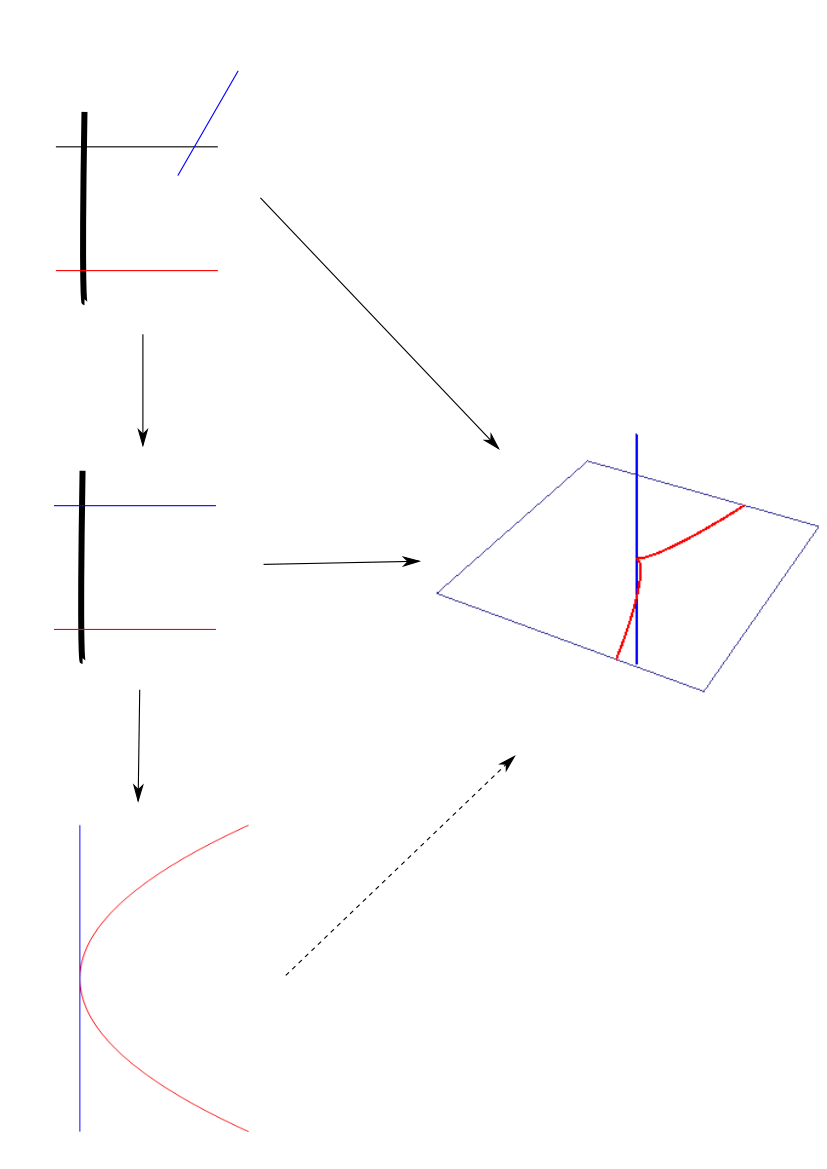
\includegraphics[width=10cm,height=5cm]{cusp_line_transv.png}
\end{center}

However Viscardi's argument can be fixed. Let $(\mathcal{C}_\eta,F_{\eta})$ be a stable map to $\PP^r$, defined on the generic point of a DVR scheme $T$; we may assume that $\mathcal C_{\eta}$ is smooth \cite[Section~3.2.1]{VISC}. 
As described in \cite[Theorem~3.6, Step~1]{VISC}, after applying nodal reduction we get a map $F\colon\mathcal C_T\to\PP^r_{T}$, for which we may suppose that $C:=\cC_0$ is and nodal and reduced $f:=F_0$ is stable.

If $f$ is not constant on the minimal genus $1$ subcurve, then it is already $m$-stable and there is nothing to say. Otherwise let $E\subset C$ be the maximal connected genus $1$ subcurve where $f$ is constant and let $R_1\sqcup\ldots\sqcup R_m=\overline{C/E}$.

 By Proposition~\ref{prop:components}~(2) we know there is a non-trivial linear relation among the $\operatorname{d}\!f(T_{q_i}R_i)$'s.
 %In other words, the first derivatives of the sections $s_0,\dots,s_r$ defining $f$, satisfy a non trivial linear relation around $q_1,\dots,q_m =E\cup\bar{C/E}$.
 Consider a maximal one with all non-zero coefficients.  Possibly after relabelling, such a relation looks like:
 \begin{equation*}\label{eq:linrelation}
 \alpha_1\operatorname{d}\!f(T_{q_{1}}R_{1})+\ldots +\alpha_j \operatorname{d}\!f(T_{q_{j}}R_{j})=0.
 \end{equation*}
 In this case we blow-up $\mathcal{C}_T$ in $q_{j+1},\ldots, q_m$. The induced map $\tilde{F_0}$ is constant on the exceptional divisors $G_{j+1},\ldots, G_m$ and we can complete the above linear relation to 
 \[\alpha_1\operatorname{d}\!\tilde f(T_{q_{1}}\tilde R_{1})+\ldots +\alpha_j \operatorname{d}\!\tilde f(T_{q_{j}}\tilde R_{j})+\beta_{j+1}\operatorname{d}\!\tilde f(T_{q_{j+1}}E_{j+1})+\ldots+\beta_m\operatorname{d}\!\tilde f(T_{q_{m}}E_m)=0\]
  with any choice of non-zero coefficients $\beta$. Now this \emph{sprouting} \cite[Section 2.3]{SMY2} ensures that the sections descend to the corresponding elliptic $m$-fold singularity. Notice that, for every $m_1\leq m_2$, there is a morphism from an $m_2$-elliptic singularity to an $m_1$-elliptic point that is birational on the target and contracts $m_2-m_1$ branches of the source to the singular point. At this point proceed with Step~2 of Viscardi's algorithm.
  
%$\operatorname{d}\!f(T_{q_i}R_i)=0$ for some $i$, say for $i\in\left\{1,\dots,j\right\}$. 
% Then blow-up $\mathcal{C}$ at $q_{j+1},\ldots, q_m$. Observe that all $\operatorname{d}\!\tilde f(T_{q_i}R_i),\ i=1,\ldots,j$ and $\operatorname{d}\!\tilde f(T_{q_i}E_i),\ i=j+1,\ldots,m$ vanish, hence they satisfy any linear relation with non-zero coefficients, and they factorise through the corresponding singularity. The map has positive degree on the first $i=1,\ldots,j$ branches.

\end{remark}

The irreducible components of Viscardi's moduli space $\overline{\pazocal{M}}^{(m)}_{1,n}(\PP^r,d)$ are also well understood \cite[Thm.~5.9]{VISC}; indeed they have a similar description to the ones of Kontsevich's space. The main advantage of the $m$-stable compactification is that the number of components drops as $m$ increases.

In particular the space $\Mone{1}{\PP^r}{d}$ we will consider in the next sections has not got the boundary component $D_{(d)}(\PP^r,d)$.
% \begin{cor}\cite[Cor.~5.10]{VISC}
% For $m\geq\operatorname{min}(r,d)+n$, $\overline{\mathcal{M}}^m_{1,n}(\PP^r,\beta)$ is irreducible.
 %\end{cor}
 
 \subsection{A different characterisation of smoothability}
 Inspired by Viscardi's alternate compactification, we give yet another characterisation of smoothable maps in genus $1.$
 \begin{dfn}
 Let $C$ be a reduced curve over $\k$ and $p\in C$ a singular point. We define the \emph{genus of the singularity} in $p$ to be the quantity: \[g(p)=\delta(p)-b(p)+1,\] where $\delta(p)=\dim_{\k}(\nu_*\OO_{\overline C}/\OO_C)\otimes k(p),$ $\nu\colon\overline{C}\to C$ is the normalisation of $C$ at $p$, and $b(p)$ is the number of branches of $C$ at $p.$
 \end{dfn}

 \begin{prop}\label{prop:smoothability2}
 Let $[f\colon C\to \PP^r]$ be a stable map from a genus $1$ curve $C=E {}_{\mathbf p}\!\sqcup_{\mathbf q}\bigsqcup_{i=1}^m R_i$, where $E$ is the maximal genus $1$ subcurve contracted by $f$, and the $R_i$'s are rational tails on which $f$ has positive degree. 
  
  Then $f$ is smoothable if and only if it factors through a Cohen-Macaulay genus $1$ singularity with positive degree on at least one of its branches.
\end{prop}

\begin{lem}(Classification of Cohen-Macaulay genus $1$ singularities)
The CM (i.e. reduced) genus $1$ singularities with $m$ branches are obtained by gluing a genus $0$ singularity with $k$ branches together with a Smyth's $(m-k)$-elliptic fold.
Notice that $k$ may be $0$ (i.e. a point) or $1$ (i.e. a smooth rational curve).
\end{lem}
\begin{proof}
We extend the argument given by Smyth \cite[Appendix~A]{SMY1} to classify the Goreinstein genus $1$ singularities. We study the analytic germ of the singularity and we adopt Smyth's notation: $R$ denotes the completion of the local ring of $C$ at the singularity; 
$\widetilde{R}=\k[[t_1]]\oplus\ldots\oplus \k[[t_m]]$ its integral closure; $\mathfrak{m}_R$ the maximal ideal of $R$  and $\mathfrak{m}_{\widetilde{R}}$ that of $\widetilde{R}.$

Let us recall that to describe $R$ as a quotient polynomial ring, it is enough to find a $\k$-basis for $\mathfrak{m}_R/\mathfrak{m}^2_R=\langle e_1,\ldots, e_s\rangle_{\k}$ where the $e_i$'s are some elements in $\widetilde{R}.$ Indeed, once given such a basis, it is a consequence of completeness that $R$ can be recognized as $\k[[x_1,\ldots, x_s]]/I$, where $I$ is the kernel of the ring homomorphism
\begin{align*}\label{eq:singularity}
\k[[x_1,\ldots, x_s]]&\rightarrow R\subset \k[[t_1]]\oplus\ldots\oplus \k[[t_m]]\\
\;\;x_i\;\; &\mapsto \;\; e_i\;\;
\end{align*}
Smyth observes that $\widetilde R/R$ is graded by:
\[ (\widetilde R/R)_i:=\mathfrak m_{\widetilde R}^i/(\mathfrak m_{\widetilde R}^i\cap R)+\mathfrak m_{\widetilde R}^{i+1}\]
Furthermore:
\begin{enumerate}
\item $m=\delta(p)=\sum_{i\geq 0}\dim_\k(\widetilde R/R)_i;$
\item $1=g(p)=\sum_{i\geq 1}\dim_\k(\widetilde R/R)_i;$
\item if $(\widetilde R/R)_i=(\widetilde R/R)_j=0$ then $(\widetilde R/R)_{i+j}=0$.
\end{enumerate}
From (3) and (2) it follows that $\dim_\k(\widetilde R/R)_1=1$ and $\dim_\k(\widetilde R/R)_i=0$ for $i\geq 2$. Then the exact sequence:
\[ 0\to \frac{\mathfrak m_{\widetilde R}^2}{\mathfrak m_{\widetilde R}^2\cap R}\to\frac{\mathfrak m_{\widetilde R}}{\mathfrak m_{\widetilde R}\cap R}\to (\widetilde R/R)_1\to 0\]
entails that:
\[\mathfrak{m}^2_{\widetilde{R}}\subseteq \mathfrak m_R,\qquad \mathfrak{m}_R/\mathfrak{m}^2_{\widetilde{R}}\subseteq \mathfrak{m}_{\widetilde{R}}/\mathfrak{m}^2_{\widetilde{R}}\;\;\text{is a codimension $1$ $\k$-subspace}.\]
Obviously $\mathfrak{m}^2_{R}\subseteq\mathfrak{m}^2_{\widetilde{R}}$. Hence $s$ is at least $m-1$. After relabelling we may assume $e_1,\dots e_{m-1}$ generate $\mathfrak{m}_R/\mathfrak{m}^2_{\widetilde{R}}$, and after Gaussian elimination they take the following form:
\begin{align*}
e_1&= (t_1, 0, \ldots, 0, a_1 t_m) \\
e_2&= (0, t_2, \ldots, 0, a_2 t_m) \\
 & \ldots \\
e_{m-1} &= (0, 0,\ldots, t_{m-1}, a_{m-1}t_m)
\end{align*}
with $a_{1}, \ldots, a_{m-1}\in \k.$ At this point Smyth restricts his attention to Gorenstein singularities and shows that under this assumption he can choose all the $a_i$ to be $1$; furthermore $\mathfrak{m}^2_{\widetilde{R}}=\mathfrak{m}^2_{R}$ holds if $m\geq 3$, thus the above are generators for $\mathfrak{m}_R/\mathfrak{m}^2_R$ and the goal is reached. For $m=1$ (resp. $2$) he finds extra generators and shows they satisfy the equation of a cusp (resp. a tacnode).

Removing the Gorenstein restriction we have three possibilities for $m\geq 3$:
\begin{enumerate}
\item At least two of the $a_i$'s are non-zero, say $i=1,2$: then $a_1a_2t_m^2=e_1\cdot e_2$ so $\mathfrak{m}^2_{\widetilde{R}}=\mathfrak{m}^2_{R}$ and we are done as above. It is easily seen that  $e_1,\ldots, e_{m-1}$ satisfy the equations of a $(k,m-k)$ singularity where $k$ is the number of $a_i$'s that are zero.
\item Only one of the $a_i$'s is non-zero, say $a_1=1$: then $\mathfrak{m}^2_{\widetilde{R}}=\mathfrak{m}^2_{R}+(t_m^2)$ and by adjoining $e_m=t_m^2$ to the $e_i$'s we see that they generate $\mathfrak{m}_R/\mathfrak{m}^2_R$ and they satisfy the equation of a tacnode $(e_1^2-e_m)e_m=0$ and $e_ie_j=0$ for $i\neq j$ and $(i,j)\neq(1,m)$, so this is an $(m-2,2)$ singularity.
\item Finally all the $a_i$'s are zero: then we have to add $t_m^2,\ t_m^3$ to generate $\mathfrak{m}_R/\mathfrak{m}^2_R$ and we obviously find an $(m-1,1)$ singularity.
\end{enumerate}
\noindent Similarly for $m=2$ there are two possibilities: the tacnode (corresponding to $a_1\neq 0$) and the union of a cusp with a non-coplanar line (for $a_1=0$), with equations:
\[ \k[[x,y,z]]/(xz,yz,y^2-x^3)\]
\noindent For $m= 1$ the only possible singularity is the cusp: indeed it can be proven that $\mathfrak{m}^2_{\widetilde{R}}=\mathfrak{m}_{R}$. 
\end{proof}

\begin{remark}
 The genus and number of branches are not sufficient to tell these singularities apart anymore, neither is the embedding dimension. A numerical invariant that distinguishes them is:
\[ \dim_\k R/I_p \]
where 
\[I_p=\operatorname{Ann}_R(\widetilde R/R)=\left\{f\in\, R\;\rvert\; f\cdot\widetilde{R}\subseteq R\right\}\]
 is the conductor ideal at the singular point. 
 Using the explicit description of $R$ given in the lemma above, we can easily find generators of $I_p$ and check that for a $(k,m-k)$ singularity we have:
 \[ \dim_\k R/I_p=m-k.\]
\end{remark}

\begin{lem}
Every Cohen-Macaulay genus $1$ singularity is smoothable.
\end{lem}
\begin{proof}
We exhibit explicit smoothings for the above singularities.
Start with two families $(\cC^0;\sigma_0,p_1,\ldots,p_k)\to T$ and $(\cC^1;\sigma_1,q_{k+1},\ldots,q_m)\to T$ respectively of smooth $(k+1)$-pointed rational curves and smooth $(m-k+1)$-pointed elliptic curves over a DVR scheme $T$, e.g. consider two trivial families.

 Then perform a blow-up along the trace of $p_1,\dots p_k$ and $q_{k+1},\dots q_{m}$ on the central fibers  $(\cC^0)_0$ and $(\cC^1)_0$ to get families $\widetilde{\cC}^0\xrightarrow{\pi_0} {\cC}^0$ and $\widetilde{\cC}^1\xrightarrow{\pi_1} {\cC}^1$ respectively.
 
We can now find semi-ample line bundles which are trivial on the strict transform of the central fiber and ample everywhere else, namely
\begin{align*}
\mathcal L_0&=\pi_0^*\OO_{\cC^0}(p_1+\ldots+ p_k)(-F_1-\ldots -F_k),\\
 \mathcal L_1&=\pi_1^*\OO_{\cC^1}(q_{k+1}+\ldots+ q_{m})(-F_{k+1}-\ldots -F_{m})
\end{align*}
where we denoted by $F_j$ the exceptional divisors of the blow-ups.

We can then use them to give contraction maps. The contracted families   $\;\hat{\cC}^0\to T\;$ and $\;\hat{\cC}^1\to T\;$ still have smooth generic fibers of genus $0$ and $1$ respectively and, by construction, $(\hat{\cC}^0)_0$ has a genus $0$ singularity with $k$ branches and $(\hat{\cC}^1)_0$ has a Smyth's $(m-k)$-elliptic point \cite[Lemma~2.12]{SMY1}.

Observe now that $\sigma_0$ and $\sigma_1$ induce sections of the contracted curves $\hat{\cC}^0\to T$ and $\hat{\cC}^1\to T$ passing through the singular points of the central fiber. Let $\hat{\cC}\to T$ the family of curves obtained by gluing $\hat{\cC}^0\to T$ and $\hat{\cC}^1\to T$ along $\sigma_0$ and $\sigma_1$ (pushout). Then $\hat{\cC}$ has a nodal generic fiber which clearly can be further smoothed.
\end{proof}

\begin{proof}\ref{prop:smoothability2}
 The argument that if $f$ is smoothable then it has to factor through a genus $1$ singularity was given by Vakil when he showed that the tangent vectors have to be linearly dependent in the image \cite[Lemma 5.9]{Vre}.
 
Viceversa, let us suppose that $f\colon C\to \PP^r$ factors through $\hat{f}\colon \hat{C}\to\PP^r$  with $\hat{C}$ a genus $1$ singularity in a way that at least one branch is not contracted.

We first show that:
\begin{claim}
 We can produce smoothings $\cC$ of $C$ and $\hC$ of $\hat C$ with a contraction map $\cC\to\hC$ compatible with the given $C\to\hat C$. See Remark \ref{rem:compatible_smoothing} below
 \end{claim}
\begin{proof}
 Assume that $\hat C$ has a $(k,m-k)$-singularity. 
Pick a smoothing $\cC$ of $C$ such that after resolving the $A_n$ singularities at the nodes, i.e. when looking at the semistable model with regular total space $\cC^{\rm{ss}}$, the following holds: call $E$ the maximal \emph{balanced} genus $1$ subcurve \cite[Proposition~2.11]{SMY1} contracted by $f^{\rm{ss}}$,
 then there are $m-k$ rational tails of positive degree directly adjacent to $E$ and the other $k$ rational tails are further away, possibly at different distances.
 %Notice that $f^{\rm{ss}}$ is defined since $C^{\rm{ss}}$ differs from $C$ only for $-2$ curves.

 We may then perform a two-step contraction: by the work of Smyth we can find a line bundle contracting $E$, namely:
\[\mathcal L=\omega_{\cC^{\rm{ss}}/T}\left( \sum_{F\subseteq E}(l+1-l(F,Z)F\right),\]
where $Z$ is the core, $l(\cdot,\cdot)$ is the distance function on the dual graph and $l$ is the maximum value attained by $l(\cdot,Z)$ on $E$. Let us call $\bar\cC$ the family of curves obtained from this contraction; notice that $f^{\rm{ss}}$ descends to a $\bar f\colon\bar\cC\to PP^r$. The central fiber $\bar{C}$ has an $(m-k+h)$-fold elliptic point with $h\leq k$, and it still has a contraction map $\rho$ to $\hat{C}$.

If necessary we may add markings $p_1+\ldots+ p_N=\Sigma$ on all the $f$-contracted rational components away from the genus $1$ singularity, and on the branches of the $(m-k+h)$-fold that are not contracted by $\rho$. Now use $\hat{f}^*\OO_{\PP^r}(1)(\Sigma)$ to perform a second contraction. Since it has no $H^1$, it satisfies cohomology and base change, and we can check that the result of this second contraction is a $(k,m-k)$-singularity simply by looking at the vanishing orders of the sections on $\bar{C}$. %These sections are constant on the branches of the singularity to which we have not added any marking, so we conclude that the dependence relation among  the tangent vectors of the branches at the singular point of the second contraction only involve the $m-k$ rational tail image of the ones adjacent to $E$.

%Since $\hat{C}$ with the added markings $\Sigma$ is stable, the morphism $\cC^{\rm{ss}}\to\cC$ we just constructed factors through a morphism
%$\cC\to\hat{\cC}$ whose central fibers are $C$ and $\hat{C}$ and compatible with $f$ and $\hat{f}.$
\end{proof}

Let $\hat{\mathcal L}$ an extension of $\hat{L}:=\hat{f}^*\OO_{\PP^r}(1)$ on $\hat{\cC}$, which exists because deforming line bundles on curves is unobstructed.
In order to extend $\hat{f}$ to $\hat{F}\colon \hat{\cC}\to\PP^r$ all we have to show is that the $r+1$ sections $\hat{s}_0,\dots, \hat{s}_{r+1}$ representing the map $\hat{f}$ extend to sections of $\hat{\mathcal{L}}.$
Thus it is enough to verify that $H^1(\hat{C},\hat{L})=0$ \cite{Wang}. Once this is done we are going to obtain the smoothing of the original map by precomposing with the contraction $F\colon\cC\to\hat{\cC}\xrightarrow{\hat F}\PP^r$.

Since all the curves we are considering are Cohen-Maculay, they have a dualising sheaf $\omega_{\hat{C}}$ such that for any line bundle $\hat{L}$
\[H^1(\hat{C},\hat{L})=(H^0(\hat{C},\hat{L}^{-1}\otimes\omega_{\hat{C}}))^{\vee}.\]
It is known \cite[IV, \S~3]{serre} that  $\omega_{\hat{C}}$ can be described as the subsheaf of $\nu_* \omega_{\overline{C}}\otimes K(\overline{C})$ (where $\nu\colon\bar C\to\hat C$ is the normalisation) satisfying: for every open $U\subseteq\hat C$ a rational $1$-form $\omega\in \nu_*\left( \omega_{\overline{C}}\otimes K(\overline{C})\right)(U)$ is a section of $\omega_{\hat C}(U)$ iff
\[\sum_{q\in \nu^{-1}(0)}\rm{Res}(\nu^*(f)\omega) =0 \quad \quad \forall f\in\OO_C(U)\]

From this description it is patent that the pullback of $\omega_{\hat C}$ to the normalisation restricts to a line bundle of degree $-1$ or $0$ on every branch, according to it being one of the $k$ or $m-k$ components. Hence it can be seen from the normalisation exact sequence and Serre duality that $H^1(\hat{C},\hat{L})=0$ as soon as $\hat L$ has positive degree on one of the branches.
 \end{proof}
\begin{remark}\label{rem:compatible_smoothing}
In general is not possible to find compatible smoothings as above: pick any genus $2$ curve with a rational tail and map it to the ramphoid cusp, a planar singularity with local equation $y^2-x^5=0$. Then a compatible smoothing can be found only if the rational tail is attached to a Weierstrass point of the genus $2$ curve, as can be seen by computing the semi-stable model of the ramphoid cusp. This example was kindly suggested to us by Prof. D.I. Smyth.

\end{remark}




\begin{remark}
It is not hard to adapt Vakil's argument \cite{Vre} to show that factoring through a genus $1$ singularity is equivalent to the tangent vectors being linearly dependent in the image.
\end{remark}
\begin{remark}
The ideas above are similar to those employed in \cite[Theorem 4.5.1]{RSPW} to show that $\pazocal{V\!Z}_{1,n}(\PP^r,d)$ is smooth, where the latter is defined by requiring the factorisation property for the map through a Smyth's singularity after sprouting.
\end{remark}





\section{From $p$-fields to the quintic threefold}
We introduce the moduli space $\Mone{1}{\PP^4}{d}^p$ of $1$-stable curves with $p$-fields, we endow it with a cosection-localised $0$-dimensional virtual class supported on a proper substack (depending on the polynomial $\w$), and we show that its degree coincides with the genus $1$ cuspidal invariants of the quintic threefold $X$ up to a sign. This is a word-by-word repetition of the arguments in \cite{CLpfields} once noticed that they carry over to the situation where we work with a family of Gorenstein (not necessarily nodal) curves. Our aim in this section is to improve the legibility of this paper by providing the non-expert reader with a r\'{e}sum\'{e} of some of the key ideas contained in \cite{CLpfields}; it can otherwise be skipped.
\subsection{Moduli of sections}
\begin{dfn}
 Let $B$ be an algebraic stack and let $\pi\colon \cC\to B$ be a flat proper morphism of finite presentation which is representable by algebraic spaces and whose geometric fibers are reduced l.c.i. curves. Let $\mathcal Z$ be an algebraic stack smooth representable and quasi-projective over $\cC$. The \emph{cone of sections} of $\mathcal Z$ over $\cC$ is a $B$-stack $\mathfrak S$ defined by:
 \[\mathfrak{S}(S\to B)=\left\{\text{sections of}\ \mathcal Z_S\to\cC_S\right\};\]

 The groupoid $\mathfrak{S}$ is an algebraic stack representable and quasi-projective over $B$ \cite[Proposition~2.3]{CL}.
 
\end{dfn}
 To fix the notation let us draw the following diagram:
 \bcd
& \mathcal Z\ar[d] \\
\cC_{\mathfrak S}\ar[r]\ar[ur,bend left,"\mathfrak e"]\ar[d,"\pi_{\mathfrak S}"] & \cC\ar[d,"\pi"] \\
\mathfrak S \ar[r] & B
\ecd
where $\mathfrak e$ denotes the universal section. 
Let us see some examples of the above construction we will be interested in. 

\subsubsection*{Direct image cones}
When $\mathcal Z=\rm{Vb}(\mathcal L)$ for a line bundle $\mathcal L$ on $\cC$, the algebraic stack  $\mathfrak{S}\to B$ representing sections of $\mathcal L$ can be constructed as:   
\[C(\pi_*\mathcal L)=\Spec_B(\R^1\pi_*\mathcal L).\]
 This is essentially because $\R^1\pi_*\mathcal L$ commutes with pullback, and it has got the desired modular interpretation by Serre duality. 

\subsubsection*{Moduli of stable maps and $1$-stable maps} 
Let $X\subseteq \PP^r$ be a projective variety and let $\mathcal Z_X$ be defined by the following cartesian diagram over $\cC$:
\bcd
\mathcal Z_X\ar[r,"/\Gm"]\ar[d,hook]\ar[dr,phantom,"\Box"] & X\times \cC\ar[d,hook] \\
\mathcal L^{\oplus r+1}\setminus 0_{\cC}\ar[r,"/\Gm"] & \PP^r\times\cC
\ecd
Then $\oM_1(X,\beta)$, the moduli space of stable maps to $X$, is an open substack of the moduli space $\mathfrak{S}_X$ of sections of $\mathcal Z_X\to\cC_{\pP}$: the morphism $\oM_1(X,\beta)\to \pP$ is given by the line bundle $f^*\OO_{\PP^r}(1)$ on the universal curve over $\oM_1(X,\beta)$, that to $\mathfrak{S}_X$ by its sections $[s_0:\ldots:s_r]$ corresponding to the universal stable map $f$, and the stability condition is an open one. This is the point of view we have already taken for $X=\PP^n$ in Proposition \ref{prop:smoothability} to describe the local equations of the moduli space of maps.

Analogously the moduli space of $1$-stable maps $\oM_1^{(1)}(X,\beta)$ can be thought of as an open inside the moduli space of sections of 
\[\widehat{\mathcal Z}_X=(\operatorname{Vb}(\widehat{\mathcal{L}}^{\oplus r+1}_{\hP})\setminus 0_{\widehat{\cC}})\times_{\PP^r} X\]
over $\widehat{\cC}_{\hP}.$

\subsubsection*{Moduli of $1$-stable maps with $p$-fields}
 In this section we denote by $\hrM$ the moduli space of $1$-stable maps $\oM_1^{(1)}(\PP^4,d)$ and by $\widehat{\mathcal P}_{\hrM}=\hL_{\hrM}^{\otimes -5}\otimes\omega_{\hat\pi_{\hrM}}.$ 
 
The moduli space of $p$-fields is defined as the cone of sections of the line bundle $\widehat{\mathcal P}_{\hrM}$ over $\hC_{\hrM}$.

\begin{dfn}
 The moduli space of $1$-stable maps with $p$-fields \[\Mone{1}{\PP^4}{d}^p:=C(\hat\pi_{\hrM,*}(\widehat{\mathcal P}_{\hrM}))\] parametrises $1$-stable maps
 \bcd
 \hC_S\ar[r,"\hat f_S"]\ar[d,"\hat\pi_S"] & \PP^4 \\
 S &
 \ecd
 with a $p$-field $\hat\psi\in H^0(\hC_S,\hat f_{S}^*\OO_{\PP^4}(-5)\otimes\omega_{\hat\pi_{S}})$.
\end{dfn}

We abbreviate $\widehat{\pazocal P}:=\Mone{1}{\PP^4}{d}^p$. Employing the above description of the moduli space of $1$-stable maps,  $\widehat{\pazocal P}$ can also be thought as an open in the moduli space of sections of the vector bundle $\rm{Vb}(\hL_{\hP}^{\oplus 5}\oplus \widehat{\mathcal P}_{\hP}). $
%\bcd
%& \rm{Vb}(\mathcal P_{\rm M})\ar[d] \\
%\hat \cC_{\pazocal P}\ar[ur,bend left,"\mathfrak e"]\ar[d,"\hat\pi_{\pazocal P}"]\ar[r] & \hC_{\rm M}\ar[d,"\hat\pi_{\rm M}"] \\
%\pazocal P \ar[r,"\PtoM"] & \rm M
%\ecd

\subsection{Obstruction theories}
Sticking to the same notation as above, the morphism $\mathfrak S\to B$ admits a relative dual perfect obstruction theory:
\[ \phi_{\mathfrak S/B}\colon \mathbb T_{\mathfrak S/B}\to \mathbb E_{\mathfrak S/B}:=\R^\bullet\pi_{\mathfrak S,*}\mathfrak e^* T_{\mathcal Z/\cC}\]
The proof of this fact is given in \cite[Proposition 2.5]{CLpfields}. We notice at this point that this results applies as well when the fibers of $\cC\to B$ are l.c.i curves, since the proof relies on general properties of obstruction theories and the cotangent complex and the fact that $\mathcal Z\to\cC$ is smooth,
but never on the specification that $\cC\to B$ be a family of \emph{nodal} curves.

Let us review the examples above:
\begin{itemize}
 \item for the direct image cone of a line bundle $\mathcal L$ the dual obstruction theory is $\mathbb E_{C(\pi_*\mathcal L)/B}=\R^\bullet\pi_*\mathcal L$;
 \item the moduli space $\hrM=\oM_1^{(1)}(\PP^4,d)$ has a dual obstruction theory relative to $\hP$ given by $ \R^\bullet\hat\pi_{\hrM,*}(\bigoplus_0^4 \hL_{\hrM})$;
 \item in the case of $1$-stable maps with $p$-fields $\widehat{\pazocal P}=\oM_1^{(1)}(\PP^4,d)^p$ we get $\mathbb E_{\widehat{\pazocal P}/\hP}=\R^\bullet\hat\pi_{\widehat{\pazocal P},*}(\hL_{\widehat{\pazocal P}}^{\oplus 5}\oplus\widehat{\mathcal P}_{\widehat{\pazocal P}}).$
\end{itemize}

There is a different obstruction theory on the moduli space of $1$-stable maps relative to $\hM$, which is the one introduced by Behrend and Fantechi for spaces of morphisms \cite[Proposition 6.3]{BF}. The two obstruction theories are compatible.
\begin{lem}
 $\hP$ is a smooth Artin stack of dimension $0$. Furthermore there is a compatible triple of dual perfect obstruction theories:
 \bcd
 \hat\PtoM^*\mathbb T_{\hP/\hM}[-1]\ar[r]\ar[d,"\wr"] &  \mathbb T_{\hrM/\hP} \ar[r]\ar[d] &  \mathbb T_{\hrM/\hM} \ar[r,"{[}1{]}"]\ar[d] & {} \\
 \R^\bullet\hat\pi_{\hrM,*}(\OO_{\hat \cC})\ar[r] & \R^\bullet\hat\pi_{\hrM,*}(\bigoplus_0^4 \hL_{\hrM})\ar[r] & \R^\bullet\hat\pi_{\hrM,*}(f_{\hrM}^* T_{\PP^4})\ar[r,"{[}1{]}"] & {}
 \ecd
 implying that $\mathbb T_{\hrM/\hP}\to \mathbb E_{\hrM/\hP}:=\R^\bullet\hat\pi_{\hrM,*}(\bigoplus_0^4 \mathcal L_{\hrM})$ gives the standard Behrend-Fantechi-Viscardi virtual class on $\hrM$.
\end{lem}
\begin{proof}
 The first statement follows from deformation theory: the projection $\hat\PtoM\colon\hP\to\hM$ is unobstructed of relative dimension $0$ and $\hM$ is a smooth Artin stack of dimension $0$, since both nodal and cuspidal singularities are l.c.i., so obstructions to their deformations are contained in $\operatorname{Ext}^2_{\OO_{\hat C}}(\Omega_{\hat C},\OO_{\hat C})=0$.
 
 The fact that $\mathbb T_{\hrM/\hM}\to \mathbb E_{\hrM/\hM}:=\R^\bullet\hat\pi_{\hrM,*}(f_{\hrM}^* T_{\PP^4})$ is a perfect obstruction theory when $\hC\to\hrM$ is a family of Gorenstein curves is proved in \cite[Proposition 6.3]{BF}.
 
 The lower row in the above diagram is induced by the Euler sequence of $\PP^4$. The middle column comes from identifying the space of stable maps as an open substack of the cone of sections (see above) of $\rm{Vb}(\bigoplus_0^4\mathcal L)$ over $\hP$. The existence of such a commutative diagram is \cite[Lemma 2.8]{CLpfields}.
 
 Finally the fact that  $\mathbb T_{\hrM/\hP}\to \mathbb E_{\hrM/\hP}:=\R^\bullet\hat\pi_{\hrM,*}(\bigoplus_0^4 \mathcal L_{\hrM})$ gives the standard virtual class for the moduli space of maps follows from functoriality of virtual pullbacks \cite{Manolache-pullback}.
\end{proof}

Next consider the moduli space of $1$-stable maps with $p$-fields $\widehat{\pazocal P}$.
\begin{lem}
 There is a compatible triple of dual perfect obstruction theories \[(\R^\bullet\hat\pi_{\widehat{\pazocal P},*}(\mathcal P_{\widehat{\pazocal P}}),\R^\bullet\hat\pi_{\widehat{\pazocal P},*}(\mathcal L_{\widehat{\pazocal P}}^{\oplus 5}\oplus\mathcal P_{\widehat{\pazocal P}}),\R^\bullet\hat\pi_{\widehat{\pazocal P},*}(\mathcal L_{\widehat{\pazocal P}}^{\oplus 5}))\] for the triangle:
 \bcd
 \widehat{\pazocal P}\ar[rr,"\hat\PtoM"]\ar[dr] & & \hrM\ar[dl] \\
 & \hP &
 \ecd
\end{lem}
\noindent This follows from the general theory of moduli of sections recalled above.

\smallskip

Notice that the virtual rank of $\mathbb E_{\widehat{\pazocal P}/\hP}:=\R^\bullet\hat\pi_{\widehat{\pazocal P},*}(\mathcal L_{\widehat{\pazocal P}}^{\oplus 5}\oplus\mathcal P_{\widehat{\pazocal P}})$ is $0$, hence it endows the moduli space of $1$-stable maps with $p$-fields with a cycle class of dimension $0$. However $\widehat{\pazocal P}$ is not proper. In the next section we describe Chang-Li's cosection (depending on the choice of $\w\in\k[x_0,\ldots,x_4]_5$) of the obstruction bundle, and show that the corresponding localised cycle is supported on the proper subtack $\Mone{1}{X}{d}$ where $X=V(\w)$ is the quintic threefold, that is the degeneracy locus of the cosection.



% Notice that the virtual rank of $\mathbb E_{\pazocal P/\hP}:=\R^\bullet\hat\pi_{\pazocal P,*}(\mathcal L_{\pazocal P}^{\oplus 5}\oplus\mathcal P_{\pazocal P})$ is $0$, hence it endows the moduli space of $1$-stable maps with $p$-fields with a cycle class of dimension $0$. In facts such a cycle is supported on a way smaller closed substack, namely $\Mone{1}{X}{d}$; this follows from the
\subsection{Cosection localisation}
Recall Kiem-Li's machinery of cosection localised virtual classes \cite[Theorem 1.1]{KLcosection}:

\begin{teo*}[Localization by cosection]\label{thm:KLlocalisation}
Let $\pazocal M$ be a Deligne-Mumford stack endowed with a perfect
obstruction theory. Suppose the obstruction sheaf $\rm{Ob}_\pazocal M$ admits a
surjective homomorphism $\sigma:\rm{Ob}_\pazocal M|_U  \to \OO_U$
over an open $U\subseteq \pazocal M$.
Let $\pazocal{M}(\sigma)=\pazocal{M}\setminus U$.
Then $(\pazocal{M},\sigma)$ has a localized virtual cycle
$$[\pazocal{M}]^{\rm{virt}}_{\rm{loc}}\in A_* \pazocal{M}(\sigma).$$
This cycle enjoys the usual properties of the virtual cycles; it relates to
the usual virtual cycle $[\pazocal{M}]^{\rm{virt}}$ via 
$[\pazocal{M}]^{\rm{virt}} = \iota_*[\pazocal{M}]^{\rm{virt}}_{\rm{loc}} \in A_*  \pazocal{M}$, where
$\iota: \pazocal{M}(\sigma)\to \pazocal{M}$ is the inclusion.
\end{teo*}

We are going to construct the cosection paralleling \cite[\S\S3.2-3.4]{CLpfields}. There is a morphism of vector bundles on $\hP$ induced by iterated tensoring of line bundles:
\[ h_1\colon\rm{Vb}(\hL_{\hP}^{\oplus 5}\oplus\widehat{\mathcal P}_{\hP})\to \rm{Vb}(\omega_{\hat\pi_{\hP}}),\quad h_1(z,p)=p\w(z_0,\ldots,z_4)\]
By differentiating it and pulling it back along the universal evaluation
\bcd
& \rm{Vb}(\hL_{\hP}^{\oplus 5})\setminus\{0\}\oplus\rm{Vb}(\widehat{\mathcal P}_{\hP})\ar[d] \\
\hC_{\widehat{\pazocal P}}\ar[ru,bend left,start anchor=north, end anchor=west,"\mathfrak e"]\ar[d,"\hat\pi_{\widehat{\pazocal P}}"]\ar[r] & \hC_{\hP}\ar[d,"\hat\pi_{\hP}"] \\
\widehat{\pazocal P} \ar[r] & \rm \hP
\ecd
%here and in future $\oplus$ at the level of geometric vector bundles means the fiber product over the base
 we obtain a cosection of the relative obstruction sheaf
\begin{equation}\label{eqn:cosection}
 \begin{split}
 \sigma_1\colon\rm{Ob}_{\widehat{\pazocal P}/\hP}=\R^1\hat\pi_{\widehat{\pazocal P},*}(\hL_{\widehat{\pazocal P}}^{\oplus 5}\oplus\widehat{\mathcal P}_{\widehat{\pazocal P}})\to \R^1\hat\pi_{\widehat{\pazocal P},*}(\omega_{\hat\pi_{\widehat{\pazocal P}}})\simeq \OO_{\widehat{\pazocal P}} \\
 \sigma_{1|(u,\psi)}(x,p)=p\w(u)+\psi\sum_{i=0}^4\partial_i\w(u)x_i
\end{split}
\end{equation}

The degeneracy locus of this cosection is $\Mone{1}{X}{d}$: by Serre duality if $\w(u)\neq 0$ then we can find a $p$ such that the cosection does not vanish; similarly we can do if $\psi\sum_{i=0}^4\partial_i\w(u)\neq 0$. But $\w(u)=0$ and $\partial_i\w(u)=0$ never happen simultaneously by smoothness of $X$, so it has to be $\psi=0$. 

Moreover Chang and Li prove that $\sigma_1$ lifts to a cosection of the absolute obstruction bundle $\rm{Ob}_{\widehat{\pazocal P}}\to\OO_{\widehat{\pazocal P}}$ with the same degeneracy locus. This is a technical expedient to show that the relative intrinsic normal cone is contained in the closed substack of the obstruction bundle determined by the cosection.

We may thus endow $\Mone{1}{\PP^4}{d}^p$ with a localised virtual cycle:
\[\virloc{\widehat{\pazocal P}}=0^{!}_{\sigma_1,\rm{loc}}[\mathfrak{C}_{\widehat{\pazocal P}/\hP}]\;\in\; A_0\left(\Mone{1}{X}{d}\right).\]

We want to show that it gives the same numerical invariants as the cuspidal Gromov-Witten theory of $X$, up to a sign:
\begin{thm}
 \[\deg[\Mone{1}{\PP^4}{d}^p]^{\rm{vir}}_{\rm{loc}}= (-1)^{5d}\deg[\Mone{1}{X}{d}]^{\rm{vir}}\]%=:GW_1^{\rm{cusp}}(X,d)\]
\end{thm}

\subsection{Sketch of the proof}
This is achieved in two steps: we first compare the invariants of $\Mone{1}{\PP^4}{d}^p$ with the ones coming from $\Mone{1}{N_{X/\PP^4}}{d}^p$, where $N_{X/\PP^4}$ is the normal bundle of the quintic in $\PP^4.$

Second we compare the latter invariants with $\deg[\Mone{1}{X}{d}]^{\rm{vir}}.$

\subsubsection*{Step~1}
This is attained in \cite[\S\S4-5]{CLpfields} by a family version of the $p$-fields construction applied to the deformation to the normal cone of $X\subseteq \PP^4$; let us denote the latter by $V\to\Aaff^1_t$, so that $V_{t\neq 0}=\PP^4$ and $V_0=N_{X/\PP^4}.$
%The idea is: construct a perfect obstruction theory for $\Mone{1}{V}{d}^p$ relative to $\hP$ which is compatible with the obstruction theories of the fibers $\Mone{1}{V_t}{d}^p;$ then construct a family version of the cosection and the fact that for compatible obstruction theories taking cosection localized cycles commutes with Gysin pull-back to conclude this Step.

\begin{lem}
 The deformation to the normal cone $V$ is cut inside $\rm{Vb}(\OO_{\PP^4}(5))\times\Aaff^1_t$ with basis coordinates $[x_0:\ldots:x_4]$ and fiber coordinate $y$ by the equation $\w(x)-ty=0$. If $C(V)$ denotes the affine cone over $V$, then its tangent bundle is determined by the following exact sequences:
 \begin{equation*}
  \begin{split}
   0\to T_{C(V)/\Aaff^1_t}\to\OO^{\oplus 5}_{C(V)}\oplus\OO_{C(V)}\xrightarrow{\sum_i\partial_i\w(x)\mathring{x_i}-t\mathring{y}}\OO_{C(V)}\to 0 \\
   0\to T_{C(V)}\to\OO^{\oplus 5}_{C(V)}\oplus\OO_{C(V)}\oplus\OO_{C(V)}\xrightarrow{\sum_i\partial_i\w(x)\mathring{x_i}-t\mathring{y}-y\mathring{t}}\OO_{C(V)}\to 0
  \end{split}
 \end{equation*}
\end{lem}
%This is just a computation in local coordinates.
This allows a description of the moduli space of maps to $V$ as the cone of sections of a certain smooth object $\mathcal Z'$ over $\hC_{\hP\times\Aaff^1}$:

\bcd
& \mathcal Z'\ar[d]\ar[r]\ar[dr,phantom,"\Box"] & V\ar[d] \\
& \rm{Vb}(\mathcal L_{\hP}^{\oplus 5})\setminus\{0\}\oplus\rm{Vb}(\mathcal L^{\otimes 5}_{\hP})\ar[d] \ar[r] & \rm{Vb}(\OO_{\PP^4}(5))\times\Aaff^1_t\\
\hC_{\oM_1^{(1)}(V)}\ar[uur,bend left,"\mathfrak e"]\ar[d,"\hat{\pi}_{\oM_1^{(1)}(V)}"]\ar[r] & \hC_{\hP\times\Aaff^1_t}\ar[d,"\hat\pi_{\hP\times\Aaff^1_t}"] & \\
\Mone{1}{V}{(d,0)} \ar[r] & \rm \hP\times\Aaff^1_t &
\ecd

Similarly $\widehat{\pazocal V}:=\Mone{1}{V}{(d,0)}^p$ can be defined as the cone of sections of $\mathcal Z:=\mathcal Z'\oplus\rm{Vb}(\widehat{\mathcal P}_{\hP})$. The general theory explained above provides an obstruction theory for $\widehat{\pazocal V}\to\hP\times\Aaff^1_t$ \cite[Proposition 4.2]{CLpfields}:

\begin{lem}
 A dual perfect obstruction theory is given by:
 \[\phi_{\widehat{\pazocal V}/\hP\times\Aaff^1_t}\colon\mathbb T_{\widehat{\pazocal V}/\hP\times\Aaff^1_t}\to\mathbb E_{\widehat{\pazocal V}/\hP\times\Aaff^1_t}:=\R^\bullet\hat\pi_{\widehat{\pazocal V}}(f_{\widehat{\pazocal V}}^*\mathcal H\oplus\widehat{\mathcal P}_{\widehat{\pazocal V}})\]
 where $f_{\widehat{\pazocal V}}\colon \hC_{\widehat{\pazocal V}}\to V$ is the universal map and $\mathcal H$ is the vector bundle on $V$ defined by the exact sequence:
 \[0\to\mathcal H\to\pr_{\PP^4}^*\left(\OO_{\PP^4}(1)^{\oplus 5}\oplus \OO_{\PP^4}(5)\right)\xrightarrow{\sum_i\partial_i\w(x)\mathring{x}_i-t\mathring{y}} \pr_{\PP^4}^*\OO_{\PP^4}(5)\to 0.\]
The restriction of $\phi_{\widehat{\pazocal V}/\hP\times\Aaff^1_t}$ to a fiber
 \[
 \widehat{\pazocal V}_c=\left\{\begin{array}{lr} \widehat{\pazocal P} & c\neq 0 \\ \Mone{1}{N_{X/\PP^4}}{d}^p & c=0 \end{array}\right.
\]
gives the standard obstruction theory of $\widehat{\pazocal V}_c\to\hP$.
\end{lem}

We would like to conclude that the restriction of the virtual cycle to the fibers is the standard virtual cycle on the fiber. The techniques of functoriality in intersection theory teach us that we should look for a triple of compatible obstruction theories for the triangle:
\bcd
\widehat{\pazocal V}_t\ar[rr,hook,"\iota_t"]\ar[dr] & & \widehat{\pazocal V} \ar[dl] \\
& \hP &
\ecd
The cone of sections interpretation provides us with an obstruction theory relative to $\widehat{\pazocal V}\to \hP$ given by:
\[
 \mathbb E'_{\widehat{\pazocal V}/\hP}:=\R^\bullet\hat\pi_{\widehat{\pazocal V}}(f_{\widehat{\pazocal V}}^*\mathcal K\oplus\widehat{\mathcal P}_{\widehat{\pazocal V}})
\]
where $\mathcal K$ is determined by the following exact sequence on $V$:
\[
 0\to\mathcal K\to\pr_{\PP^4}^*\left(\OO_{\PP^4}(1)^{\oplus 5}\oplus \OO_{\PP^4}(5)\oplus\OO_{\PP^4}\right)\xrightarrow{\sum_i\partial_i\w(x)\mathring{x}_i-t\mathring{y}-y\mathring{t}} \pr_{\PP^4}^*\OO_{\PP^4}(5)\to 0
\]
Of course $h^0(\mathbb E'_{\widehat{\pazocal V}/\hP})\simeq\mathbb T_{\widehat{\pazocal V}/\hP}$, but the previous lemma and the difference between $\mathcal H$ and $\mathcal K$ hint at the fact that the obstruction sheaf $h^1 (\mathbb E'_{\widehat{\pazocal V}/\hP})$ contains one factor $\R^1\hat\pi_{\widehat{\pazocal V},*}\OO_{\hC_{\widehat{\pazocal V}}}\simeq \OO_{\widehat{\pazocal V}}$ too many, so that restricting $\mathbb E'_{\widehat{\pazocal V}/\hP}$ to the fibers we would not find their standard obstruction theory. A confirmation of this fact is given by observing that $\mathbb E'_{\widehat{\pazocal V}/\hP}$ equips $\widehat{\pazocal V}$ with a $0$-dimensional cycle, while we are looking for a $1$-dimensional cycle such that restricting to any fiber, i.e. applying $\iota_t^!,$ we get $[\widehat{\pazocal V}_t]^{\rm{vir}}\in A_0(\widehat{\pazocal V}_t)$.

This issue is solved in \cite[\S\S4.5-6]{CLpfields} by lifting the standard obstruction theory $\phi'_{\widehat{\pazocal V}/\hP}$ to a different, specifically tailored one: 
\[\phi_{\widehat{\pazocal V}/\hP}\colon\mathbb T_{\widehat{\pazocal V}/\hP}\to\mathbb E_{\widehat{\pazocal V}/\hP},\]
 where the latter two-term complex fits into an exact triangle:
\[ \R^1\hat\pi_{\widehat{\pazocal V},*}\OO_{\hC_{\widehat{\pazocal V}}}[-2]\to\mathbb E_{\widehat{\pazocal V}/\hP}\xrightarrow{\nu}\mathbb E'_{\widehat{\pazocal V}/\hP}\xrightarrow{[1]}\]
Furthermore the lifted obstruction theory is compatible with the standard one for the fibers.
\begin{lem}
For every $c\in\k$ we have a commutative diagram:\marginpar{the lower one is not exact}
\bcd
\hat{\pi}_{\widehat{\pazocal V}_c *}\OO_{\hC_{\widehat{\pazocal V}_c}}[-1]\ar[r] & \mathbb E_{\widehat{\pazocal V}_c/\hP} \ar[r] &\mathbb E_{\widehat{\pazocal V}/\hP}\rvert_{\widehat{\pazocal V}_c}\\
\mathbb{T}^{\geq 1}_{\widehat{\pazocal V}_c/\widehat{\pazocal V}}\ar[u]\ar[r] & \mathbb{T}^{\geq 1}_{\widehat{\pazocal V}_c/\hP}\ar[u]\ar[r] & \mathbb{T}^{\geq 1}_{\widehat{\pazocal V}/\hP}\rvert_{\widehat{\pazocal V}_c} \ar[u]
\ecd
\end{lem}
For the proof see \cite[\S~4.6]{CL}.

%Since we are working with cosection localised cycles, this is not yet enough to conclude.
 A family version of the cosection is induced by differentiating the following vector bundle morphism on $\hP\times\Aaff^1_t$:
\[
 \rm{Vb}(\hL_{\hP}^{\oplus 5}\oplus\hL_{\hP}^{\otimes 5}\oplus\widehat{\mathcal P}_{\hP})\xrightarrow{(\pr_2,\pr_3)}\rm{Vb}(\hL_{\hP}^{\otimes 5}\oplus\widehat{\mathcal P}_{\hP})\xrightarrow{\cdot}\rm{Vb}(\omega_{\hat\pi_{\hP}})
\]
The cosection takes then the following form:
\[\bar\sigma_{1|(u,v,\psi)}(\mathring{x},\mathring{y},\mathring{p})=\psi\mathring{y}+v\mathring{p}\]
It is showed in \cite[\S4.7]{CLpfields} that $\bar\sigma_1$ lifts to a cosection $\bar\sigma\colon \rm{Ob}_{\widehat{\pazocal V}}\to \OO_{\widehat{\pazocal V}}$ and that the degeneracy locus of $\bar\sigma$ is 
\[\Mone{1}{X}{d}\times\Aaff^1_t.\]

Recall that the sections $(x,y)$ are required to satisfy $\w(x)-ty=0$. So $\bar\sigma_1$ coincides up to a non-zero scalar with the above defined cosection $\sigma_1$ for $\widehat{\pazocal P}$ when $t\neq 0$. It is proved in \cite[Theorem 5.2]{KLcosection} that, given compatible perfect obstruction theories, the construction of a cosection localised virtual cycle is compatible with Gysin pullbacks, so that by \cite[Proposition 4.9]{CLpfields}:
\[
 \iota_{t\neq0}^![\widehat{\pazocal V}]^{\rm{vir}}_{\rm{\bar\sigma}}=[\widehat{\pazocal P}]^{\rm{vir}}_{\rm{\sigma}}\in A_0(\widehat{\pazocal Q}),\quad \iota_{0}^![\widehat{\pazocal V}]^{\rm{vir}}_{\rm{\bar\sigma}}=[\Mone{1}{N_{X/\PP^4}}{d}^p]^{\rm{vir}}_{\rm{\bar\sigma_0}}\in A_0(\widehat{\pazocal Q})
\]
where we have denoted by $\widehat{\pazocal Q}:=\Mone{1}{X}{d}$.
\subsubsection*{Step~2}
We are left with proving that $\deg[\Mone{1}{N_{X/\PP^4}}{d}^p]^{\rm{vir}}_{\rm{\bar\sigma_0}}$ coincides up to sign with $\deg[\Mone{1}{X}{d}]^{\rm{vir}}$.
In the rest of the section we use the following notation: $\widehat{\pazocal N}:=\Mone{1}{N_{X/\PP^4}}{d}^p$, and $\hat v\colon\widehat{\pazocal N}\to\widehat{\pazocal Q}$. 
We now find a perfect obstruction theory for $\hat v\colon\widehat{\pazocal N}\to\widehat{\pazocal Q}$ compatible with the ones of $\widehat{\pazocal N}\to\hP$ and $\widehat{\pazocal Q}\to\hP$, and then use a cosection-localised version of Manolache's virtual pullback construction~\cite{Manolache-pullback}.

Indeed Chang and Li proved that there is a perfect obstruction theory 
\[\mathbb E_{\widehat{\pazocal N}/\widehat{\pazocal Q}}:=\R^{\bullet}\hat\pi_{\widehat{\pazocal N},*}(\hL^{\otimes 5}_{\widehat{\pazocal N}}\oplus \widehat{\mathcal P}_{\widehat{\pazocal N}})\]
 compatible with $\mathbb E_{\widehat{\pazocal N}/\hP}$ and $\hat v^*\mathbb E_{\widehat{\pazocal Q}/\hP}$, so that $\mathbb E_{\widehat{\pazocal N}/\widehat{\pazocal Q}}$ inherits a cosection $\sigma_0'$ with degeneracy locus $D(\sigma_0')=\widehat{\pazocal Q}$. Then in \cite[Lemma 5.5]{CLpfields} they show by using the techniques of \cite{KKP} that $\mathfrak C_{\widehat{\pazocal N}/\widehat{\pazocal Q}}$ is supported inside 
\[
 h^1/h^0(\mathbb E_{\widehat{\pazocal N}/\widehat{\pazocal Q}})_{\sigma_0'}:=\operatorname{Ker}(\sigma_0')\cup  h^1/h^0(\mathbb E_{\widehat{\pazocal N}/\widehat{\pazocal Q}})\rvert_{D(\sigma_0')}
\]
so that they may combine the techniques of virtual pullback \cite{Manolache-pullback} and localisation by cosection \cite{KLcosection} to define:
\[
 \hat v^!_{\mathbb E_{\widehat{\pazocal N}/\widehat{\pazocal Q}},\rm{loc}}\colon A_*(\widehat{\pazocal Q})\to A_*(D(\sigma_0')=\widehat{\pazocal Q})
\]
sending $[\widehat{\pazocal Q}]^{\rm{vir}}$ to $[\Mone{1}{N_{X/\PP^4}}{d}^p]^{\rm{vir}}_{\rm{\bar\sigma_0}}.$

To conclude it is now enough to compute the degree of $\hat v^!_{\mathbb E_{\widehat{\pazocal N}/\widehat{\pazocal Q}},\rm{loc}}.$
Since we are only interested in what happens to $A_0(\widehat{\pazocal Q})$, we just need to compute $\deg(\hat v^!_{\mathbb E_{\widehat{\pazocal N}/\widehat{\pazocal Q}},\rm{loc}}[\zeta])$ for a closed point $\zeta$. This is done in \cite[Theorem 5.7]{CLpfields} and the same considerations work in our case.
%They notice that the fibers of $v$ are vector spaces and the obstruction theory $\mathbb E_{\pazocal N/\widehat{\pazocal Q}}$ is symmetric, so it can be represented as 
%\[[T_{v^{-1}(\xi)}\xrightarrow{0}T^*_{v^{-1}(\xi)}]\] along the fibers. This is enough since we are only interested in the action of $v^!_{\mathbb E_{\pazocal N/\widehat{\pazocal Q}},\rm{loc}}$ on $A_0(\widehat{\pazocal Q})$ \cite[Theorem 5.7]{CLpfields}.

Hopefully we have managed to convince the reader that the subtle intersection theory perpetuated in \cite{CLpfields} does not rely at all on the hypothesis that the families of curves we are working with are \emph{nodal}, but \emph{l.c.i.} curves are well-behaved enough so that all the proofs carry over to the situation of our interest.







\section{The comparison morphism}
%In this section we start investigating the Gromov- Witten type invariant obtained from Viscardi compactification studying the case $m=1$: the source curve is at worst cuspidal. We will see how in this case we can give a comparison with the GW-invariant and explain why the same technique does not work for higher $m$.
%The first thing we do is the following:
%we introduce a moduli space of stably-weighted, prestable, at worst cuspidal, marked curves. We show that there is a birational morphism from a correspondingly decorated moduli space of prestable nodal curves. Taking the fiber product with Viscardi's moduli space of stable cuspidal maps, we show that the resulting space includes in the usual Kontsevich's moduli space, precisely avoiding the component with elliptic tails $D_{\{d\},\{n\}}(X,d)$.

%Why should such a morphism on decorated prestable curves exist? 
%Consider an elliptic tail $C$; a one-dimensional family $\mathcal C$  with central fiber $\mathcal C_0\cong C$ will either be locally constant or smoothen the node. In the first case we can associate to this the locally constant family of cusps obtained by forgetting the elliptic tail and contracting a length-two infinitesimal neighborhood of the node in the rational component; in the second case, we claim that the line bundle $\mathcal O_\mathcal C(3q)$ gives a morphism to a smoothing of the cuspidal $\PP^1$. This heuristics (i.e. being able to substitute an elliptic tail with a cusp over points or DVR schemes) motivates us to believe we can define a morphism from suitably defined moduli spaces of nodal genus one curves to cuspidal curves (cfr. \cite[Lemma 4.2]{SMY2}). In fact we shall extend \cite[Corollary 4.5]{SMY2} to an appropriate setup of moduli stacks of weighted prestable curves. Assume $d>0$ throughout the following.
In this section we shall:
\begin{itemize}
 \item argue in two different ways that there is a natural fashion to associate a weighted $1$-stable curve to a weighted-stable nodal curve of genus $1$, essentially by replacing elliptic tails of weight $0$ by cusps, which results in a morphism:
 \[\mathfrak M_{1,n}^{\operatorname{wt},\text{st}}\to\mathfrak M_{1,n}^{\operatorname{wt},\text{st}}(1)\]
extending the identity on the locus of smooth elliptic curves;
 \item introduce the fiber product 
 \[\Z:= \mathfrak M_{1,n}^{\operatorname{wt},\text{st}}\times_{\mathfrak M_{1,n}^{\operatorname{wt},\text{st}}(1)} \oM^{(1)}_{1,n}(\PP^4,d)\]
 and show that it is a closed substack of $\oM_1(\PP^4,d)$, isomorphic to it outside the boundary divisor $D^1$;
 \item introduce the fiber product \[\Zp:=\mathfrak M_{1,n}^{\operatorname{wt},\text{st}}\times_{\mathfrak M_{1,n}^{\operatorname{wt},\text{st}}(1)} \oM^{(1)}_{1,n}(\PP^4,d)^p \]
 and endow it with an obstruction theory and a cosection thereof, which are pulled back from  $\pazocal M^{(1)}_{1,n}(\PP^4,d)^p$; unfortunately we will not be able to compare them directly with $\oM_1(\PP^4,d)^p$;
 \item explain along the way all the notation one needs in order to understand the previous sentences.
\end{itemize}
%in two different ways that there exists a morphism at the level of weighted prestable curves $\mathfrak M_{1,n}^{\operatorname{wt},\text{st}}\to\mathfrak M_{1,n}^{\operatorname{wt},\text{st}}(1);$ introduce the spaces 
%\[\Z:= \mathfrak M_{1,n}^{\operatorname{wt}=d,\text{st}}\times{\mathfrak M_{1,n}^{\operatorname{wt}=d,\text{st}}(1)} \pazocal M_{1,n}(\PP^4,d)(1),\qquad \Zp:=\mathfrak M_{1,n}^{\operatorname{wt}=d,\text{st}}\times{\mathfrak M_{1,n}^{\operatorname{wt}=d,\text{st}}(1)} \pazocal M^p_{1,n}(\PP^4,d)(1) \]
%and  and see their relation, respectively, with the moduli space of stable maps, stable maps with fields; use the morphism at the level of prestable curves to induce obstruction theories on $\Z$ and $\Zp.$


Note that the only type of nodal curves that we are getting rid of are the ones with an elliptic tail of weight zero.

\begin{thm}
There exists a morphism $\mathfrak M_{1,n}^{\operatorname{wt}=d,\text{st}}\to\mathfrak M_{1,n}^{\operatorname{wt}=d,\text{st}}(1)$ which extends the identity on the smooth locus.
\end{thm} 
As anticipated we explain two different approaches to the proof:
\begin{enumerate}
 \item we adopt the strategy of constructing the graph of such a morphism within the product $\mathfrak M_{1,n}^{\operatorname{wt}=d,\text{st}}\times\mathfrak M_{1,n}^{\operatorname{wt}=d,\text{st}}(1)$ and prove that the projection onto the first factor is an isomorphism;
\item we prove that the $1$-stabilisation exists at the level of curves with a divisor constructing the contraction directly, then argue that it descends to a morphism between moduli spaces of weighted curves.
\end{enumerate}

\subsection{First approach: the graph}

Let $\mathcal C$ and $\mathcal C'$ be the universal curves over $\mathfrak{M}:=\mathfrak M_{1,n}^{\operatorname{wt}=d,\text{st}}$ and $\mathfrak{M}':=\mathfrak M_{1,n}^{\operatorname{wt}=d,\text{st}}(1)$ respectively. Abusing notation, we will still write $\mathcal C$ and $\mathcal C'$ for their pullbacks to the product $\mathfrak{M}\times\mathfrak{M}'$ along the two projections. The proof of the theorem follows from two Lemmas:

\begin{lem}\label{lemma:def_X}
 There is a locally closed substack $\mathcal X\subseteq\operatorname{Mor}_{\mathfrak{M}\times\mathfrak{M}'}(\mathcal C,\mathcal C')$ representing morphisms $C\to C'$ that contract weight-zero elliptic tails to cusps and are weight-preserving isomorphisms everywhere else. 
\end{lem}

\begin{lem}\label{lamma:projection_iso}
 The first projection $\pr_1\colon \operatorname{Mor}_{\mathfrak{M}\times\mathfrak{M}'}(\mathcal C,\mathcal C')\to\mathfrak M$ restricted to $\mathcal X$ is an isomorphism with $\mathfrak M$.
\end{lem}

\begin{proof}\ref{lemma:def_X}
Recall that $\operatorname{Mor}_{\mathfrak{M}\times\mathfrak{M}'}(\mathcal C,\mathcal C')$ is an algebraic stack; in fact the map to $\mathfrak{M}\times\mathfrak{M}'$ is representable (by algebraic spaces) \cite{OlssonHOM}. We now proceed to construct $\mathcal X$ as a locally closed substack in the space of morphisms.

\begin{description}[labelindent=0cm,leftmargin=\parindent]

\item[Step 1] Consider
 \[\pi\colon\mathfrak{P}=\mathfrak{Pic}^{tot deg=d,st}_{1,n}\to\mathfrak{M},\ \pi'\colon\mathfrak{P}'=\mathfrak{Pic}^{tot deg=d,st}_{1,n}(1)\to\mathfrak{M}'\]
  the Picard stacks of $\cC\to\mathfrak{M}$ and $\cC'\to\mathfrak{M'}$ with universal line bundles $\mathfrak{L}$ and $\mathfrak{L'}$, where $\pi$ and $\pi'$ are defined by taking the multi-degree of line bundles. We can now look at the algebraic stack $\operatorname{Mor}_{\mathfrak{P}\times\mathfrak{P}'}(\mathcal C,\mathcal C')$ with universal morphism
 $\Phi$ and natural projection $\Pi$ to $\operatorname{Mor}_{\mathfrak{M}\times\mathfrak{M}'}(\mathcal C,\mathcal C')$. We claim that there exists a locally closed substack $\mathcal{Y'}\subseteq \operatorname{Mor}_{\mathfrak{P}\times\mathfrak{P}'}(\mathcal C,\mathcal C')$ representing those morphisms that \emph{preserve the line bundles}. Indeed, given a chart 
 \begin{equation*}%\label{equation:Spoints} 
 S\to\operatorname{Mor}_{\mathfrak{P}\times\mathfrak{P}'}(\mathcal C,\mathcal C'),
  \end{equation*} 
   the locus of $s\in S$ where $\Phi_s^*\mathfrak{L}'_s\cong\mathfrak{L}_s$ is nothing else than the locus $T$ where the two sections $\mathfrak{L}_S$ and $\Phi_S^*\mathfrak{L}'_S$ of $\mathfrak{P}(S)\to\mathfrak{M}(S)$ coincide. In other words, we are looking at the fiber product 
  \[\xymatrix{T\ar[r]\ar[d]&\mathfrak{P}\ar[d]^{\Delta}\\
  S\ar[r]&\mathfrak{P}\times_{\mathfrak{M}}\mathfrak{P}}\]
Being $\mathfrak{P}\to\mathfrak{M}$ representable by locally separated algebraic spaces \cite[Theorem~8.3.1]{neron}, $\Delta$ is a quasi-compact locally closed immersion \cite[\href{http://stacks.math.columbia.edu/tag/04YU}{Tag 04YU}]{stacks-project}, so in particular $T\subseteq S$ is locally closed.

\item[Step 2] 
Furthermore there is a closed substack $\mathcal Y\subseteq \mathcal Y'$ representing \emph{surjective morphisms that preserve the markings}.

Given a chart $S\to\operatorname{Mor}_{\mathfrak{P}\times\mathfrak{P}'}(\mathcal C,\mathcal C')$, the locus of $s\in S$ where $\Phi_s$ is marking-preserving is the equaliser of the two sections
\bcd
S \ar[r,shift left, "\times\sigma_i'" above]\ar[r,shift right,"\times\Phi\circ\sigma_i" below] & \mathcal C_S'\times_S\ldots\times_S \mathcal C_S'
\ecd
This defines a closed subscheme of $S$, since $\mathcal C_S'\to S$ is separated.

As regards surjectivity, since $\Phi$ is proper and the dimension of the fiber is upper semicontinuous \cite[\href{http://stacks.math.columbia.edu/tag/0D4I}{Tag 0D4I}]{stacks-project}, the locus in $\mathcal C_S'$ where the fiber of $\Phi$ is empty is open. Its image in $S$ is open by flatness of $\cC'\to S$ \cite[\href{http://stacks.math.columbia.edu/tag/01UA}{Tag 01UA}]{stacks-project}, and the complement of it is the locus we need.
 
\item[Step 3] Let $\mathcal{X}'$ be the image of $\mathcal Y$ under $\Pi$. This is a constructible substack of $\operatorname{Mor}_{\mathfrak{M}\times\mathfrak{M}'}(\mathcal C,\mathcal C')$ by Chevalley's theorem \cite[Theorem 5.9.4]{LMB}. Recall that to show that a constructible set is open (respectively closed) it is enough to check that it contains all the generisations of its points (respectively all the specialisations) \cite[\href{http://stacks.math.columbia.edu/tag/0DQN}{Tag 0DQN}\href{http://stacks.math.columbia.edu/tag/0903}{Tag 0903}]{stacks-project}. Finally, under Noetherian assumptions, two points related by specialisation/generisation are contained in the image of a DVR scheme \cite[\href{http://stacks.math.columbia.edu/tag/054F}{Tag 054F}]{stacks-project}.

It is clear that being surjective and marking-preserving are closed conditions, as above. The requirement that $\phi$ can be covered by a line bundle-preserving map can be translated into the following combinatorial conditions:

\begin{enumerate}
\item\emph{$\phi$ contracts only weight zero components.} We show that this is open. Assume that $S$ is a DVR scheme with closed point $0$ and generic point $\eta$, and we are given $S\to\mathcal X'$ such that $\phi_0\colon\mathcal C_0\to \mathcal C_0'$ does not contract any positive weight component. Suppose there exists an irreducible component $D_\eta\subseteq C_{\eta}$ of positive weight $d_W$ which is contracted by $\phi_{\eta}.$ The contracted locus, i.e. $\left\{c\in \mathcal{C}_{S} | \dim_c\phi^{-1}(\phi(c))\geq 1\right\}$, is closed by semicontinuity of fiber dimension, hence it contains all the components $D_i\subseteq C_0$ to which $D_\eta$ specialises. At least one of them has positive weight, since the sum of their weights is $d_W$, which is a contradiction.

\item\emph{$\phi$ has degree 1 on every non contracted component} or, equivalently, there is an $S$-dense open in $\mathcal C'_S$ such that the restriction of $\phi_S$ to its preimage is an isomorphism.
This is an open and closed condition; we show it is open. Let $S$ be a DVR scheme as above and assume that $\phi_0$ satisfies the property. Since $\phi_S$ is proper, we may consider 
\[\phi_{S,*}[\mathcal C_{S}]=\sum n_i[\mathcal C'_{S,i}]\in A_2(\cC'_S)\]. Applying Gysin pull-back to $0$ (which is a regular closed point of the base) \cite[Prop. 10.1(a)]{FUL}, we see that all the $n_i$'s are 1 for those $\cC'_i$'s such that $0^![\cC'_i]\neq 0$. On the other hand there is no irreducible component of $\cC'$ supported on $\cC'_\eta$.

\item\emph{$\phi$ is weight-preserving.} This is again an open condition, as we can see from the weighted dual graphs. Let $\tilde \phi$ be the map induced at the level of weighted dual graphs $\Gamma(\cC)\to\Gamma(\cC')$. It is compatible with the specialisation maps:
\bcd
\Gamma(\cC_0)\ar[r,"\tilde\phi_0"]\ar[d,"\rm{sp}"] & \Gamma(\cC'_0)\ar[d,"\rm{sp}"] \\
\Gamma(\cC_{\eta})\ar[r,"\tilde\phi_\eta"]& \Gamma(\cC'_\eta)
\ecd
Since the weight of a component of the generic fiber is determined by those of the components to which it specialises
\[ \deg(v)=\sum_{w\in\rm{sp}^{-1}(v)}\deg(w)
\]
$\tilde{\phi}_\eta$ has to be weight-preserving as well.
\end{enumerate}

\item[Step 4] We have seen that, if $\phi$ contracts a connected subcurve $E$ of the fiber, it must have zero weight. Since the target only has nodes and cusps as singularities, and the markings are required to be smooth points, we observe that $E$ must be of arithmetic genus one by weighted stability and $|\overline{C\setminus E}\cap E|\leq 2$, i.e. $E$ is either an elliptic tail or an elliptic bridge. There are basically two possibilities:
\begin{enumerate}
\item $\phi$ contracts an elliptic tail to a cusp and is an isomorphism everywhere else, or there is no elliptic tail to start with and $\phi$ is an isomorphism;
\item the elliptic tail/bridge is contracted to a smooth point/node, then a non-separating node or a cusp must be created somewhere else in order to preserve the arithmetic genus.
\end{enumerate} 
We want to avoid the second scenario, so we define the open substack $\mathcal X\subseteq \mathcal X'$ as follows.
Given $\mathcal{C}_S\to\mathcal C_S'\in\mathcal X'(S)$, let $U'\subseteq \mathcal C'$ be the \emph{maximal} $S$-dense open subset such that $\phi_S|_{\phi_S^{-1}(U')}\colon\phi_S^{-1}(U')\to U'$ is an isomorphism and $Z'$ its closed complement in $\mathcal C_S'$. 
Then $\mathcal X$ is the open locus \cite[\href{http://stacks.math.columbia.edu/tag/055G}{Tag 055G}]{stacks-project} where the fibers of $\pi|_{\phi^{-1}(Z')}\colon \phi^{-1}(Z')\to S$ are geometrically connected.
\end{description} 
 \end{proof}
 
 \begin{proof}\ref{lamma:projection_iso}
 This result will follow from an application of Zariski's Main Theorem for algebraic spaces.
First we claim that the projection is \emph{representable by algebraic spaces}: by \cite[\href{http://stacks.math.columbia.edu/tag/04Y5}{Tag 04Y5}]{stacks-project} we only need to check that it is faithful, and by \cite[Theorem 2.2.5]{CONR} it is enough to look at geometric points. Hence we need to say that, given $\phi\colon C\to C'$ a $k$-point of $\X$, we have
$\operatorname{Aut}(\phi)\subseteq\operatorname{Aut}(C)$. Recall that automorphisms of $\phi$ are commutative diagrams:
\bcd C\ar[r,"\phi"]\ar[d,"\psi"] & C'\ar[d,"\psi'"] \\ C\ar[r,"\phi"] & C' \ecd
 Now $\psi'$ is determined by $\psi$ due to our description of $\phi$.
 
Secondly $\pr_{1|\mathcal X}$ is \emph{proper}: this can be seen using the valuative criterion
\bcd
\eta'=\Spec(K')\ar[r]\ar[d] & \eta=\Spec(K)\ar[r]\ar[d] & \mathcal X \ar[d] \\
S'=\Spec(R')\ar[r]\ar[urr,dashed,"\exists?", left] & S=\Spec(R)\ar[r] & \mathfrak M
\ecd
Let $\pi \colon \mathcal C_S\to S$ be the family of nodal curves on $S$; there are three cases to consider:
\begin{enumerate}
\item the central fiber contains no elliptic tail, then the same is true for $\mathcal C_\eta$, hence $\phi_\eta$ is an isomorphism. We can extend $\phi_\eta$ as follows:
\bcd
\cC_\eta\arrow{r}{\sim}[swap]{\phi_\eta}\ar[d,hook,"\iota"] & \cC'_\eta\ar[d,hook,"\iota\circ\phi_\eta^{-1}"] \\
\cC_S\ar[r,"\id_\cC"] & \cC_S=:\cC'_S
\ecd
Another extension $\phi'\colon \mathcal C_S\cong \mathcal C_S'$ would be isomorphic to the previous one via:
\bcd
\cC_S\ar[r,"\phi'"]\ar[d,"\id"] &\cC_S'\ar[d,"(\phi')^{-1}"] \\
\cC_S\ar[r,"\id"] & \cC_S
\ecd

\end{enumerate}
If instead $\mathcal C_0$ has got an elliptic tail, then we have two possibilities:
\begin{enumerate}
\setcounter{enumi}{1}
\item $\mathcal C_{\eta}$ has an elliptic tail as well; that is the image of $S\to\MM$ is contained in the boundary, so we can find a lift
\bcd
 & \MM_{1,1}\times\MM_{0,1+n}^\text{wt}\ar[d] & \\
 S\ar[r]\ar[ur,dashed] & \mathfrak D_{\{1,\emptyset\},\{0,n\}}\ar[r,hook] &\MM.
\ecd
 Then $\mathcal C_S$ is the push-out of a family of rational curves $\mathcal R_S$ and a family of genus one curves $\mathcal Z_S$:
%The map $S\to\partial \mathfrak M_{1,n}$ lifts to the normalisation of the boundary, i.e. $\mathfrak M_{0,n_0+1}\times\mathfrak M_{1,n_1+1}$, which gives two families of pointed curves on $S$; there is a map from the push-out to $\mathcal C_S$ by the universal property, and it is proper bijective and flat (crit\`{e}re de platitude par fibres \cite[\href{http://stacks.math.columbia.edu/tag/039A}{Tag 039A}]{stacks-project}).
\begin{equation}\label{eq:pushout}
\begin{tikzcd}
S\ar[d]\ar[r] & \mathcal R_S \ar[d] \\
\mathcal Z_S\ar[r] & \mathcal C_S
\end{tikzcd}
\end{equation}
Recall that the cuspidal curve $\cC'_K$ can be characterised as the push-out of the following diagram:
\bcd
2K\ar[r]\ar[d] & \mathcal R_K\ar[d] \\
K\ar[r] & \mathcal C'_K.
\ecd
Since the smooth section $S\to\mathcal R_S$ defines a Cartier divisor, it makes sense to take its double and we can thus define $\cC'_S$ by means of the similar diagram:
\bcd
2S\ar[r]\ar[d] & \mathcal R_S\ar[d] \\
S\ar[r] & \mathcal C'_S
\ecd
The morphism $\phi_S\colon\cC_S\to\cC'_S$ extending $\phi_\eta$ is then defined by exploiting the description of $\cC_S$ as a push-out \eqref{eq:pushout}, and the morphisms $\id\colon\mathcal R_S\to \mathcal R_S$ and $\pr_{\mathcal Z_S}\colon\mathcal Z_S\to S$.
\item If $\mathcal C_S$ smoothens the elliptic tail, then $\phi_\eta$ is an isomorphism. We may assume that $S$ is the spectrum of a complete DVR with algebraically closed residue field \cite[Theorem 7.10]{LMB}. Then we may pick one smooth section for each rational component of $\cC_0$ and extend them to sections of $\cC_S\to S$ by Grothendieck's existence theorem; let us denote by $\Sigma$ the Cartier divisor that is the sum of all such sections. Let $Z$ be the elliptic tail in the central fiber; then we claim that $\omega_{\cC_S/S}(Z)\otimes\mathcal O_{\cC_S}(\Sigma)$ is $\pi_S$ semi-ample, ample on the generic fiber, and gives the contraction of the elliptic tail to the cusp in the central fiber. We shall not prove the claim here, since this is the core of the second approach.
\end{enumerate}
Finally, observe that the map is bijective by construction and $\mathfrak M$ is normal, hence $\pi_{|\mathcal X}\colon\mathcal X\to \mathfrak M$ is an isomorphism by Zariski's main theorem (as in \cite[\href{http://stacks.math.columbia.edu/tag/082I}{Tag 082I}]{stacks-project}).
 \end{proof}
 
\subsection{Second approach: constructing the contraction}

The idea behind this construction is essentially due to Hassett \cite[\S2]{HassettHyeon} and it has recently been reviewed and simplified in \cite[\S3.7]{RSPW}.

Let $\mathfrak{P}=\mathfrak{Pic}^{d,rm{st}}_{\cC/\MM_1}$ with the stability condition that the line bundle $\omega_\pi\otimes \mathcal L^{\otimes 3}$ on the universal curve is $\pi$-relatively ample. 

We work over $\MM_1^{\rm{div}}$, parametrising families of nodal curves with a relative Cartier divisor. More precisely, this can be thought of as the open inside $C(\pi_*\mathcal L)=\Spec_\pP(\R^1\pi_*\mathcal L)$ (see \cite{CLpfields} and Section \ref{section:p-fields} above), where the section of $\mathcal L$ is not $0$ on any irreducible component of the curve. Alternatively this is the moduli functor of a prestable curve with a line bundle and a section up to scalar, which can be thought of as the hom-stack $\Hom_{\MM_1}(\mathcal C,[\Aaff^1/\Gm])$; then again one picks the connected component where the line bundle has total degree $d$, and the open substack obtained by requiring weighted stability and the section not to vanish on any irreducible component of the curve.

We shall construct the contraction over $\MM_1^{\rm{div}}$ first, and then show that it descends to $\MM_1^{\rm{wt}}$.

Let $E$ be the locus inside the universal curve spanned by elliptic tails of weight $0$; this is a Cartier divisor in the universal curve over $\MM^{\rm{wt}}_1$, which we shall freely pullback and keep denoting by $E$. We shall also denote by $\mathfrak D^1$ its image in $\MM^{\rm{wt}}_1$ (and its various pullbacks), which is a Cartier divisor as well.

Consider the following line bundle on the universal curve over $\MM_1^{\rm{div}}$: 
\begin{equation}\label{eq:linebundlecontraction}
\mathcal N:=\omega_{\pi}(E)\otimes\mathcal O_{\cC}(3D),
\end{equation} where $D$ is the universal Cartier divisor over $\MM_1^{\rm{div}}$ (so $\mathcal O_{\cC}(D)$ is the pullback of the universal line bundle on $\pP$).
Notice that $\mathcal N$ is trivial on the locus of elliptic tails, so the Proj construction applied to it will contract this locus.

\begin{prop}\label{1-stabilization-div}
In the following diagram $\hC$ is a family of weighted $1$-stable curves and $\phi$ is a regular morphism:
 
 \bcd
 (\cC,D)\ar[rr,"\phi"]\ar[dr,"\pi"] & & (\hC=\operatorname{Proj}_{\MM_1^{\rm{div}}}(\bigoplus_{n\geq 0}\pi_*\mathcal N^{\otimes n}),\phi(D))\ar[ld,"\hat\pi"] \\
 & \MM_1^{\rm{div}} &
 \ecd
This defines the $1$-stabilisation morphism $\MM_1^{\rm{div}}\to\MM_1^{(1),\rm{div}}$.
\end{prop}

We need to prove that $\mathcal N$ is $\pi$-semi-ample (regularity of $\phi$) and that $\pi_*\mathcal N$ is locally free (flatness of $\hat\pi$). Both these facts are clear generically, but less so on points of $E$ and $\mathfrak D^1$. We shall check this by exploiting the next lemma, which is a nice technical gadget drawn from \cite{RSPW}: it implies that the $\Proj$ construction we perform commutes with base-change to generic curves inside $\MM_1^{\rm{div}}$, allowing us to work with a smoothing of the elliptic tail over a DVR scheme $T$.

\begin{lem}[pullback with a boundary]\label{DVR}
Let $\pi\colon\cC\to S$ be a proper family of curves over a smooth basis, and let $\mathcal N$ be a line bundle on $\cC$ such that $\R^1\pi_*\mathcal N$ is a line bundle supported on a Cartier divisor $\mathfrak D\subseteq S$. Then for every spectrum of a DVR $T$ with closed point $0$ and generic point $\eta$, and for every morphism $f\colon T\to S$ such that $f(0)\in\mathfrak D$ and $f(\eta)\in S\setminus\mathfrak D$ we have
\[f^*\pi_*\mathcal N\cong \pi_*f^*\mathcal N.\]
%We have denoted with $\mathfrak{D}^1$ the Cartier divisor image of the locus spanned by elliptic tails.
\end{lem}
\begin{proof}
The argument can be found in \cite[Lemmma~3.7.2.2]{RSPW}.
\begin{color}{gray}{
Let $K^{\bullet}$ the complex of locally free sheaves on $S$ which satisfy cohomology and base change, i.e. such that for any $T\xrightarrow{f} S$  we get
$H^i(f^*K^{\bullet})=\R^i\pi_*f^*\mathcal M.$ The construction of $K^{\bullet}$ is standard, (see e.g. \cite[Proposition~12.2]{HAR} and since the cohomology is concentrated in degree 0,1, we can assume $K^{\bullet}=K_0\to K_1.$ Let $f$ be the map defined in the statement of the Lemma.
Then we have the following exact sequences:
\begin{equation}\label{eq:exact1}
0\to \pi_*\mathcal M\to K^0\to K^1\to \R^1\pi_*\mathcal M\to 0,
\end{equation}
\begin{equation}\label{eq:exact2}
0\to \pi_*f^*\mathcal M\to f^*K^0\to f^*K^1\to \R^1\pi_*f^*\mathcal M\to 0.
\end{equation}
The derived pull-back $Lf^*$ of the complex~\eqref{eq:exact1} is zero since the complex is exact. Writing down explicitly the spectral sequence which compute the derived pull-back, we find that its convergence to zero implies that:
\begin{align*}
\operatorname{coker}(f^*\pi_*\mathcal M\to\pi_*f^*\mathcal M)&\cong \rm{L}_1f^*\R^1\pi_*\mathcal M\\
\operatorname{ker}(f^*\pi_*\mathcal M\to\pi_*f^*\mathcal M)&\cong \rm{L}_2f^*\R^1\pi_*\mathcal M.
\end{align*} 
To prove that $\rm{L}_if^*\R^1\pi_*\mathcal M=0$ for $i=1,2$ it is enough to work locally on $S$, where we have a free resolution for  of the form $\R^1\pi_*\mathcal M$ of the form:
\[0\rightarrow \OO_S\xrightarrow{g}\OO_S\rightarrow \R^1\pi_*\mathcal M\rightarrow 0\] 
and thus pulling back along $f$
\[0\rightarrow  \rm{L}_1f^*\R^1\pi_*\mathcal M \to \OO_T\xrightarrow{f^*g}\OO_T\rightarrow f^*\R^1\pi_*\mathcal M\rightarrow 0.\] 
It immediately follows that $ \rm{L}_2f^*\R^1\pi_*\mathcal M=0.$ Finally notice that since the image of $f$ is not contained in the boundary divisor $f^*g\neq 0$ and thus injective of sheaves as $T$ is a DVR. We can then conclude $ \rm{L}_1f^*\R^1\pi_*\mathcal M=0$ as well which implies the Lemma.}\end{color}
\end{proof}
Now recall that in our case $\mathcal N$ is trivial on elliptic tails and of positive degree everywhere else. The rank of $\R^1\pi_*\mathcal N$ can be checked on the fibers \cite[Theorem III.12.11]{HAR}, so we see that it is $0$ outside $\mathfrak D^1$ and $1$ on it.

\begin{lem}\label{lemma:semiample}
The line bundle $\mathcal N$ is $\pi$-semi-ample, i.e. the natural map
\[\pi^*\pi_*\mathcal N^{\otimes n}\to \mathcal N^{\otimes n}\]
is surjective for $n\gg 0$ (in fact $n=1$ suffices).
\end{lem}
\begin{proof}
Outside the locus of elliptic tails $\mathcal N$ is $\pi$-ample. We are left to check on points belonging to an elliptic tail; thanks to the above Lemma we can reduce to the case that $C$ is the central fiber of a one-parameter smoothing of the elliptic tail. This has been dealt with by Smyth~\cite[Lemma~2.12]{SMY1}.
\end{proof}

\begin{lem}
$\pi_*\mathcal N$ is locally free on $\MM_1^{\rm{div}}.$
\end{lem}
\begin{proof}\cite[Proposition~3.7.2.1]{RSPW}
We have to check that $\pi_*\mathcal N$ has constant rank.
On $\MM_1^{\rm{div}}\setminus \mathfrak{D}^1$ we see that $\R^1\pi_*\mathcal N=0$, so $\pi_*\mathcal N$ satisfies Cohomology and Base Change and its rank is determined by Riemann-Roch.
Given a point $x$ on the boundary $\mathfrak{D}^1$, we can pick a DVR scheme $T$ whose closed point maps to $x$ and whose generic point maps to $\MM_1^{\rm{div}}\setminus \mathfrak{D}^1.$ Then we are in the hypotheses of Lemma~\ref{DVR} and we can check the rank at $x$ by looking at $\pi_*f^*\mathcal N$ over $T.$ Now $f^*\mathcal N$ is flat over $T$, so $\pi_*f^*\mathcal N$ is as well, which implies torsion-free (constant rank).
\end{proof}

\begin{proof}\ref{1-stabilization-div}
Let $S\to \MM_1^{\rm{div}}$ be a smooth atlas, then we have:
 \bcd
 (\cC_S,D_S)\ar[rr,"\phi"]\ar[dr,"\pi"] & & (\hat \cC_S=\operatorname{Proj}_{S}(\bigoplus_{n\geq 0}\pi_{S,*}\mathcal N^{\otimes n}),\phi(D_S))\ar[ld,"\hat\pi"] \\
 & S &
 \ecd
where $\phi$ is a proper and birational morphism since $\mathcal N$ is $\pi$-semi-ample and $\hat{\pi}$ is flat since $\pi_*\mathcal N$ is locally free. 
To verify that this defines a morphism $S\to \MM_1^{\rm{div}}(1)$ we have to argue that $\hat{\cC}_S$ has reduced fibers and only nodes and cusps as singularities.

Since these properties only concern the fibers of $\hat{\pi}$ we can verify them after base change to a DVR scheme $T$ chosen as in Lemma~\ref{DVR}, so that the construction commutes with base change. Furthermore we can pick $f\colon T\to S$ such that the total space $\cC_T$ is regular, so we may just apply Smyth's Contraction Lemma~\cite[Lemma~2.13]{SMY1}.

Finally to conclude that this defines a morphism 
\[\MM_1^{\rm{div}}\to \MM_1^{\rm{div}}(1)\]
it is enough to verify that there is an isomorphism
 $\rm{pr}_1^*\hat \cC_S\cong\rm{pr}_2^*\hat \cC_S$ satisfying the cocycle condition, where $\rm{pr}_i\colon S'= S\times_{\MM_1^{\rm{div}}} S\rightrightarrows S$.%and that $\rm{pr}_{ij}\colon S\times_{\MM_1^{\rm{div}}} S\times_{\MM_1^{\rm{div}}} S\to  S\times_{\MM_1^{\rm{div}}} S $ satisfy the cocycle condition.

 This follows from the fact that $\pr_i^*\hat \cC_S$ are obtained from applying the Proj construction to 
 $\rm{pr}_i^*\pi_{S,*}\mathcal{N}\cong\pi_ {S',*} \rm{pr}_i^*\mathcal N$, by flatness of $S'\to S$. Thus it is enough to show that 
 \[\rm{pr}_1^*\mathcal N\cong \rm{pr}_2^*\mathcal N.\]
  But $\mathcal N$ is the pullback of a line bundle on $\MM_1^{\rm{div}}$, thus the desired isomorphism follows from the commutativity of the diagram
 
 \bcd
S\times_{\MM_1^{\rm{div}}} S\ar[r,"\rm{pr_1}"]\ar[d, "\rm{pr_2}"] & S\ar[d] \\
S\ar[r] & \MM_1^{\rm{div}}
\ecd
 
The cocycle condition is derived similarly. 
\end{proof}


\begin{prop}
The $1$-stabilisation just defined for curves with a divisor induces an analogue morphism on weighted curves:
\bcd
\MM_1^{\rm{div}}\ar[r]\ar[d]\ar[dr,phantom,"\curvearrowright"] & \MM_1^{\rm{div}}(1)\ar[d] \\
\MM_1^{\rm{wt}}\ar[r,"\exists"] & \MM_1^{\rm{wt}}(1)
\ecd
\end{prop}
\begin{proof}
{\'E}tale locally on $\MM_1^{\rm{wt}}$ we can choose smooth sections $s_i$ of the universal curve in a way that their sum as a relative Cartier divisor $D$ has degree compatible with the weight function, so in particular it makes $\omega_{\pi}(E)\otimes\mathcal O_{\cC}(3D)$ trivial on the elliptic tails and $\pi$-ample elsewhere.
If $S\to \MM_1^{\rm{wt}}$ is a smooth atlas, up to taking an {\'e}tale cover we can assume there are sections $s_i$ of $\cC_S\to S$ that define a lifting $S\to \MM_1^{\rm{div}}$, and thus a morphism $\xi\colon S\to  \MM_1^{\rm{wt}}(1)$ through the above construction.

In order to show that this descends to a morphism $\MM_1^{\rm{wt}}\rightarrow \MM_1^{\rm{wt}}(1)$ we need to verify that  $\rm{pr}_1^*(\xi)\cong\rm{pr}_2^*(\xi)$ and the cocycle condition is satisfied, where $\rm{pr}_i\colon S'= S\times_{\MM_1^{\rm{wt}}} S\rightrightarrows S$.

This boils down to checking that for two different choices of a lifting $D_1,D_2\colon S\to\MM_1^{\rm{div}}$ there exists a unique isomorphism 
\[\hat{\mathcal C}_1=\operatorname{Proj}_S\left((\omega_{\pi}(E)\otimes\mathcal O_{\cC}(3D_1))^{\otimes n}\right)\cong \operatorname{Proj}_S\left((\omega_{\pi}(E)\otimes\mathcal O_{\cC}(3D_2))^{\otimes n}\right)=\hat{\mathcal C}_2. \]
By construction there is a birational map $\psi$
 \bcd
&\cC_S \ar[dl,"\phi_1" above left]\ar[dr,"\phi_2"]  \\
 \hat{\mathcal C}_1\ar[rr,dashed, "\psi"] & &\hat{\mathcal C}_2.
 \ecd

We want to show that $\psi$ extends to a regular morphism. 
Notice that $ \hat{\mathcal C}_i$ is normal, $i=1,2$. Indeed since $S$ is smooth and the singularities of the fibers are in codimension $1$, $ \hat{\mathcal C}_i$ is regular in codimension $1$. Moreover since both $S$ (smooth) and the fibers (Cohen-Macaulay) satisfy Serre's condition $S_2$, so does the total space of $\hC_i$ by \cite[Thorem~23.9]{MAT}. Then, since the geometric fibers of $\phi_i$ are either points or $p_a=1$ subcurves, and in either case connected, Zariski's connectedness theorem implies that
\[\phi_{i,*}\OO_{\cC_S}\cong \OO_{\hat{\mathcal C}_i}. \]
 Moreover by construction $\operatorname{Exc}(\phi_1)=\operatorname{Exc}(\phi_2)$ is the locus of elliptic tails of weight $0$, so in particular $\phi_2$ contracts all fibers of $\phi_1.$ Then \cite[Lemma 1.15]{debarre}
implies that $\phi_2$ factors through $\phi_1$, and viceversa. This proves the regularity of $\psi$ and its inverse. Notice that $\psi$ is unique as it is the only extension of $\phi_2\circ\phi_1^{-1}$.
\end{proof} 

\subsection{Fiber products and induced obstruction theories}
Let $\Z$ be defined by the pullback diagram:
\bcd
\Z \ar[r]\ar[d]\ar[rd,phantom,"\Box"] & \overline{\mathcal M}_1^{(1)}(\PP^4,d) \ar[d] \\
\mathfrak M_1^{\rm{wt}}\ar[r] & \mathfrak M_1^{\rm{wt}}(1)
\ecd

Objects of $\Z$ over $S$ consist of diagrams
\bcd
C \ar[rr,"\phi"]\ar[dr,"\pi" below left] & & \hat C\ar[rr,"f"]\ar[dl,"\hat\pi"] & & \PP^4 \\
& S & & &
\ecd
where $f$ is a $1$-stable map and $\phi$ is the weighted $1$-stabilisationdefined above (i.e. contraction of elliptic tails of weight $0$); arrows over $\id_S$ are commutative diagrams
\bcd
C\ar[r,"\phi"]\ar[d,"\psi"] &  \hat C\ar[r,"f"]\ar[d,"\hat\psi"] & \PP^4 \ar[d,"\id_\PP"]\\
C'\ar[r,"\phi'"] &  \hat C'\ar[r,"f'"] & \PP^4

\ecd
where $\psi$ and $\hat\psi$ are isomorphisms.  Recall that $\hat \psi$ is determined by $\psi$. %due to the required commutativity with the dominant ``birational'' morphism $\phi$.

Forgetting $\hat C$ and keeping $f\circ\phi\colon C\to\PP^4$, we obtain a morphism $i\colon\Z\to\oM_1(\PP^4,d).$ 

\begin{lem}
The morphism $i\colon\Z\hookrightarrow\oM_1(\PP^4,d)$ is a closed immersion. In particular $\Z$ is a proper DM stack.
\end{lem}
\begin{proof}
From the above description of arrows in $\Z$, $i$ is  representable (i.e. faithful)  and a monomorphism (i.e. full).

We can check properness using the valuative criterion. We argue as in \cite[Theorem 4.3]{RSPW}. Let $T$ be a DVR scheme with generic point $\eta;$ consider a diagram:
\bcd
\cC_{\eta}\ar[r]\ar[d,"\phi_{\eta}" left]  & \cC_T\ar[d,"\phi_T" left]\ar[r,"f"] & \PP^4 \\
\hat{\cC}_{\eta}\ar[r,"j" below]\ar[urr] & \hat{\cC_T}\ar[ur,dashed ,"g" below right] &
 \ecd 
Notice that there is an open dense substack of $\Z$ where $\phi$ is an isomorphism. Indeed the generic point of either the main component or any boundary component is already $1$-stable. Thus we can assume that $\phi_{\eta}$ in the above diagram is an isomorphism.

Observe that $f$ is constant on the fibers of $\phi_T$, so it factors topologically through $\hat{\cC}.$
We can conclude as in \cite{RSPW} or appeal to \cite[Lemma~1.15]{debarre} using $\phi_*\OO_{\cC_T}\cong\OO_{\hat{\cC}_T}$. To see this consider the exact sequence:
\[0\to \OO_{\hat{\cC}_T}\to\phi_*\OO_{\cC_T}\to \phi_*\OO_{\cC_T}/\OO_{\hat{\cC}_T}\to 0\]
Since $\phi$ is an isomorphism away from the cuspidal point, the cokernel is supported in dimension $0$. However $\chi (\OO_{\hat{\cC}_\eta})=\chi(\phi_*\OO_{\cC_\eta})$ implies the same equality holds on the whole of $T$, since the Euler characteristic is constant in flat families. So $\chi(\phi_*\OO_{\cC_T}/\OO_{\hat{\cC}_T})=\operatorname{length}(\phi_*\OO_{\cC_T}/\OO_{\hat{\cC}_T})=0.$
\end{proof}


So we may add the commutative diagram to the left:
\bcd
\oM_1(\PP^4,d)\ar[d] & \pazocal Z \ar[l,hook,swap,"i"]\ar[r]\ar[d]\ar[rd,phantom,"\Box"] & \overline{\mathcal M}_1^{(1)}(\PP^4,d) \ar[d] \\
\MM^{\rm{wt}}_1 & \X\ar[l,swap,"\sim"]\ar[r] & \mathfrak M_1^{\rm{wt}}(1)
\ecd


From the inclusion $i$ we easily obtain a description of the irreducible components of $\Z$: there is a main component $\Z^\text{main}$ which is the closure of the locus of maps from a smooth elliptic curve, and for every $k\geq 2$ a boundary component $D^k\Z$, whose general point represents a contracted elliptic curve with $k$-many rational tails of positive degree. 

Notice that the above lemma means that each and every component of $\Z$ is isomorphic to the corresponding one in $\oM_1(\PP^4,d)$. Indeed given any stable map there is at most one factorisation through the weighted $1$-stabilisation of the curve: objects of $\oM_1(\PP^4,d)\setminus D^1$ are $1$-stable already; objects of $D^1\cap \oM_1(\PP^4,d)^\text{main}$ do factor through the cusp thanks to Vakil's criterion, which implies the node joining the elliptic tail to the rational tail of positive degree is a ramification point of the map; and objects of $D^1\cap D^k$ ($k\geq 2$) do factor through a map which is constant on the cusp.\marginpar{insert figure of a typical element of $D^1\cap D^2$.} On the other hand, objects of $D^{1,\circ}=D^1\setminus(\oM_1(\PP^4,d)^\text{main}\cup\bigcup_{k\geq 2}D^k)$ do not admit any factorisation, so $\Z$ has no corresponding component.

We introduce two more relevant spaces: let $\XP$ and $\Z^p$ be the algebraic stacks defined by the following cartesian diagram:
\bcd
\Z^p \ar[r,"\alpha"]\ar[d]\ar[rd,phantom,"\Box"] & \overline{\mathcal M}_1^{(1)}(\PP^4,d)^p \ar[d] \\
\XP \ar[r]\ar[d]\ar[rd,phantom,"\Box"] & \mathfrak{Pic}_1{(1)} \ar[d] \\
\X\ar[r] & \mathfrak M_1^{\rm{wt}}(1)
\ecd

The obstruction theory $\R^\bullet\hat{\pi}_*(\hat{\mathcal L}^{\oplus 5}\oplus\widehat{\mathcal P})$ for the morphism $\overline{\mathcal M}_1^{(1)}(\PP^4,d)^p\to\mathfrak{Pic}_1{(1)}$ together with its cosection induce a localised virtual class on $\Z^p$ by virtual pullback of $[\XP]$. In Section \ref{section:main_proof} we shall conduct on this a similar analysis to that in \cite{CL} and compare the contribution of the main component to Vakil-Zinger's reduced invariants.

\begin{remark}
The stack $\XP$ parametrises
\bcd
C\ar[rr,"\phi"]\ar[dr] & & \hat C\ar[ld] \\
& S &
\ecd
with a line bundle $\hat{\mathcal L}$ on $\hat{C}$. Notice that by pulling back $\hat{\mathcal L}$ via $\phi$ we obtain a line bundle on $C$, hence a morphism $\XP\to \mathfrak{Pic}_1$. This is generically an isomorphism, but has $1$-dimensional fibers over the locus of elliptic tails, due to the fact that $\Pic(\hat C)\to\Pic(C)$ has kernel $\mathbb G_{\rm a}$ when $\hat C$ has a cusp.
\end{remark}
On the other hand notice that
\[ \X\times_{\mathfrak M_1^{\rm{wt}}(1)} \mathfrak M_1^{\rm{div}}(1) \to \mathfrak M_1^{\rm{div}} \]
is an isomorphism. We just check on points.
\marginpar{I am not sure, CHECK ME.}
\begin{comment}
Given a line bundle $\mathcal L$ on $C$ and a section $s_0\in\Gamma(C,\mathcal L)$  there is exactly one line bundle $\hat{\mathcal L}$ on the $1$-stabilisation of $C$ and one section $\hat s_0\in\Gamma(\hat C,\hat{\mathcal L})$ that pull back to $(\mathcal L,s_0)$.
Let us denote with $p$ the node separating the elliptic tail and the $\PP^1$, which we think as pointed normalisation $\nu\colon(\PP^1,p)\to \hat C$ of the cusp. There are just two cases to be consider: $s_0$ does not vanish on the elliptic curve; the section is identically $0$ on $E$. 

In the first case, $\nu(s_0\rvert_{\PP^1})$ is a smooth divisor $\hat{D}_0$ in $\hat$ and the line bundle $\OO_{\hat{C}}(\hat{D}_0)$ together with the defining section equation $\hat{s}_0$ of the smooth sub-scheme  $\nu(s_0\rvert_{\PP^1})$ pull-back to $\mathcal L$ and $s_0.$

If $D_0$ contains the node, notice that since $p$ is not Cartier in $C$, the section $s_0$ vanishes in $p$ at least with order two, i.e.  
\end{remark}

\begin{lem}\marginpar{CHECK ME}
Let $\nu\colon(\PP^1,p)\to \hat C$ be the pointed normalisation of the cusp. Then $0\neq s\in\Gamma(\PP^1,\OO_{\PP^1}(d))$ with $s(p)=0$  determines a unique line bundle $\hat{\mathcal L}$ on $\hat C$ to which $s$ descends  only if $s'(p)=0$.
\end{lem}
\begin{proof}
The key point is that the sections of $\hat{\mathcal L}$ pull back to a $d$-dimensional subspace of $\Gamma(\PP^1,\OO_{\PP^1}(d))$ that can be identified as follows: they are those sections $\sigma$ such that $s(p)\sigma'(p)=s'(p)\sigma(p)$ in any trivialisation of $\OO_{\PP^1}(d)$ near $p$ if $s(p)\neq 0$, and those constant to second order at $p$ otherwise.
\end{proof}
\end{comment}

\begin{remark}
Similarly the stack $\Z^p$ parametrises
\bcd
C\ar[rr,"\phi"]\ar[dr,"\pi" below left] & & \hat C\ar[ld,"\hat\pi"] \ar[r,"f"] & \PP^4\\
& S & &
\ecd
with a $p$-field $\psi\in H^0(\hat C,f^*\OO_{\PP^4}(-5)\otimes\omega_{\hat\pi})$.

We were not able to compare $\Z^p$ with $\oM_1(\PP^4,d)^p$ directly, since denoting by $\hat{\mathcal L}=f^*\OO_{\PP^4}(1)$ and by $\mathcal L=\phi^*\hat{\mathcal L}$ we only have a map $\R^1\hat\pi_*\hat{\mathcal L}\to\R^1\pi_*\mathcal L$ on $\Zp$ which is not an isomorphism (dually, since $\phi^*\omega_{\hat\pi}=\omega_{\pi}(E)$, the $p$-fields on $C$ that we get by pulling back from $\hat C$ vanish on elliptic tails).
\end{remark}

As anticipated we may endow $\Z^p$ with a localised virtual cycle by ``localised virtual pullback''.
Indeed, consider on $\Z^p$ the perfect obstruction theory $\mathbb E_{\Z^p/\XP}:=\alpha^*\left(\mathbb E_{\Mone{1}{\PP^4}{d}^p/\mathfrak{Pic_1{(1)}}}\right)$ and the induces cosection
\[\alpha^*\sigma\colon \OO b_{\Z^p/\XP}\to \Z^p\]
whose degeneracy locus is
\[\pazocal D(\alpha^*\sigma)=\pazocal D(\sigma)\times_{\Mone{1}{\PP^4}{d}^p} \Z^p.\]
Then we have that
\begin{align*}
\mathfrak C_{\Z^p/\XP}& \subseteq \alpha^*\mathfrak C_{\Mone{1}{\PP^4}{d}^p/\mathfrak{Pic_1{(1)}}}\\
& \subseteq \alpha^* h^1/h^0\left(\mathbb E_{\Mone{1}{\PP^4}{d}^p/\mathfrak{Pic_1{(1)}}}\right)_\sigma\\
&\cong h^1/h^0\left(\mathbb E_{\Z^p/\XP}\right)_{\alpha^*\sigma}
\end{align*}
and we can thus define $[\Z^p]^{\rm{vir}}_{\alpha^*\sigma,\rm{loc}}.$
\begin{color}{red}
\begin{lem}
localised virtual pullback commutes with pushforward. In particular,
\[\alpha_* [\Z^p]^{\rm{vir}}_{\alpha^*\sigma,\rm{loc}}=[{\Mone{1}{\PP^4}{d}^p}]^{\rm{vir}}_{\sigma,\rm{loc}}\] 
\end{lem}
\end{color}
\marginpar{check \cite{KLcosection}, probably needs the proper morphism to be surjective}

\begin{cor}
$\deg[\Z^p]^{\rm{vir}}_{\rm{loc}}=\deg[\Mone{1}{\PP^4}{d}^p]^{\rm{vir}}_{\rm{loc}}$
\end{cor}








\section{Local equations and desingularisation}\label{sec:equations}
\subsection{Equations for $\Z^p$ relative to $\XP$}
We are going to need a description of the normal cone $\mathfrak C_{\Z^p/\XP}$ in order to perform a splitting.

Since $\Z^p$ simply is a line bundle over the boundary of $\Z$, we may instead find equations for the latter.

Recall that $\Z$ can be embedded as an open inside $C(\hat{\pi}_*\mathcal L^{\oplus 5})$ over $\XP$. We are going to find an embedding of $C(\hat{\pi}_*\mathcal L^{\oplus 5})$ in a smooth ambient space over $\XP$, that will be a vector bundle obtained by suitably twisting $\mathcal L$.

Following \cite{HL}, we work locally on $\Z$: start with a point $\xi=[(C\xrightarrow{\phi}\hat C\xrightarrow{f}\PP^4]\in\Z$ and choose coordinates on $\PP^4$ such that $f^{-1}\{x_0=0\}$ is a simple smooth divisor $D=\sum_{i=1}^d\delta_i$ on $\hat C$. This continues to be true on a neighbourhood $U$.

 Locally the morphism $\Z\to\XP$ can be written as $\xi\mapsto[C\to\hat C,\OO_{\hat C}(D)]$, which admits a local lifting $U\to\MM_1^{(1),\rm{div}}$ and in fact hits the smooth locus of the latter.
 
  Notice though that the projection $\MM_1^{(1),\rm{div}}\to \XP$ (or to $\Pic_1^{(1)}$ for what it is worth) is \emph{not} smooth. In fact, when the line bundle is trivial on the minimal elliptic subcurve $E$, it may be deformed to a degree $0$, non-effective line bundle on such a subcurve, so that sections of $\OO_{\hat C}(D)$ which are constant and non-zero on $E$ are obstructed.

There is a way around this: in a neighbourhood $V\subseteq \XP$ of $[C\to\hat C,\OO_{\hat C}(D)]$ we can write the universal line bundle $\mathcal L_V$ as $\OO_{\hC_V}(\pazocal D + p-p_0)$. Indeed we can pick a local section $p_0$ through the minimal genus $1$ subcurve, so that $\mathcal L_V(p_0)$ becomes effective. We should then think of $p$ as a local coordinate on $\XP$ relative to $\X$.

Locally on $V$ we can pick another smooth section $\A$ of the minimal genus $1$ subcurve not intersecting $p_0$, neither the support of $\pazocal D+p$.

\begin{lem}
$C(\hat\pi_*\mathcal L)$ is the kernel of the vector bundle map:
\[ \hat\pi_*\OO_{\hC}(\A+\pazocal D+p-p_0)\xrightarrow{\varphi}\hat\pi_*\OO_{\A}(\A)\]
Up to shrinking $V$ we may write:
\[\hat\pi_*\OO_{\hC}(\A+\pazocal D+p-p_0)\cong\bigoplus_{i=1}^d\hat\pi_*\OO_{\hC}(\A+\pazocal \delta_i+p-p_0)\oplus\hat\pi_*\OO_{\hC}(\A+p-p_0)\]
\end{lem}
Compare with \cite[Lemma 4.10]{HL}. Denote by \[\varphi_i\colon\hat\pi_*\OO_{\hC}(\A+\pazocal \delta_i+p-p_0)\to\hat\pi_*\OO_{\A}(\A)\] (and similarly $\varphi_p$) the composite of the inclusion with $\varphi$.

Let us introduce some more notation: around a point $[\hat C]\in\MM_1^{(1),\rm{wt}}$, for every node $q$ of $\hat C$ there is a coordinate $\zeta_q$ whose vanishing locus is the divisor where such a node is \emph{not} smoothed. These functions can be pulled back to $V$. Denote by \[\zeta_{[\delta_i,a]}=\prod\zeta_q\]
where the product runs over all the nodes separating $\delta_i$ from the minimal genus $1$ curve.
 
\begin{lem}
We may find an explicit local expression for $\varphi_i$ and $\varphi_p$ after trivialising the relevant line bundles:
\[\varphi_i=\zeta_{[\delta_i,a]}, \quad \varphi_p=(p-p_0)\]
\end{lem}
Compare with \cite[Proposition 4.13]{HL}.
\begin{remark}
The vanishing locus of $(p-p_0)$ on the boundary means that the line bundle restricts to the trivial one on the minimal genus $1$ subcurve. The meaning of it is not clear outside the boundary.
\end{remark}

\begin{lem}\label{lem:equations}
A local chart $U$ for $\Z$ can be embedded as an open inside:
\[ (F_0=\ldots=F_4=0)\subseteq \rm{Vb}(\hat{\pi}_*\mathcal L^{\oplus 5}) \]
where
\[ F_j=\sum_{i=1}^d \zeta_{[\delta_i,a]}w_i^j+(p-p_0)w_{d+1}^j \]
and $w_i^j$ are coordinates on the fiber of the $j$-th copy of $\rm{Vb}(\hat{\pi}_*\mathcal L)$ over $\XP$.
\end{lem}
Compare with \cite[Theorems 2.17-19]{HL}.

\subsection{Hu-Li blow-up and desingularisation}
We perform a modular blow-up of $\MM_1^{1,\rm{wt}}$: we successively blow up $\hat\Theta_k, \;k\geq 2$  defined as the closure of the loci where the minimal elliptic subcurve $E$ has weight $0$ and $\lvert\overline{C\setminus E}\cap E\rvert=k.$

Notice that after the $k$-th blow-up, the strict transform of $\Theta_{k+1}$ is smooth, so the final result  $\widetilde{\MM}_1^{1,\rm{wt}}$ is smooth as well. 

\begin{remark}
The fiber product 
\[\widetilde{\MM}_1^{1,\rm{wt}}\times_{\MM_1^{1,\rm{wt}}}\MM_1^{\rm{wt}}\]
recovers the Hu-Li blow-up $\widetilde{\MM}_1^{\rm{wt}}.$ The key observation is that $\Theta_1$ is already a Cartier divisor and the pullback of $\hat\Theta_k$ is precisely $\Theta_k$.
\marginpar{you can use the universal property of the blow up to show there are maps in both directions. Check the statement about the $\Theta_k$}
\end{remark}

\begin{remark}\label{rmk:eqn}
After blowing up, the equations in \ref{lem:equations} are simplified and assume the following form:
\[\tilde\zeta\tilde w+(p-p_0)w_{d+1}=0\]
where $\tilde\zeta$ is one of the newly created boundary divisors $\widetilde{\Theta_k}$ from $\widetilde{\MM}_1^{\rm{wt}}$ (i.e. one of the exceptional divisors produced by the blow-up process), and $\tilde w$ is a suitably defined coordinate on the fiber of $\rm{Vb}(\hat{\pi}_*\mathcal L)\times_{\XP}\widetilde{\XP}$.
\end{remark}

Summing up, we get:
\bcd
   &  \widetilde{\Z}^p \ar[r]\ar[d]\ar[rd,phantom,"\Box"] & \tM_1^{(1)}(\PP^4,d)^p \ar[d] \\
\tM_1(\PP^4,d)\ar[d] & \widetilde{\Z} \ar[l,hook,swap,"i"]\ar[r]\ar[d]\ar[rd,phantom,"\Box"] & \tM_1^{(1)}(\PP^4,d) \ar[d] \\
\widetilde{\mathfrak{Pic}}_1\ar[d] &\widetilde{\XP}\ar[l]\ar[r]\ar[d]\ar[rd,phantom,"\Box"] & \widetilde{\mathfrak{Pic}}_1 ^{(1)}\ar[d]\\
\widetilde{\MM}^{\rm{wt}}_1 & \widetilde{\X}\ar[l,swap,"\sim"]\ar[r] & \widetilde{\MM}_1^{(1),\rm{wt}}
\ecd




\begin{comment}
where this time an object of $\Z^p$ over $S$ is given by
\bcd
\cC\ar[rr,"\phi"]\ar[dr,"\pi"] & & \hat\cC\ar[rr,"f"]\ar[dl,"\hat\pi"] & & \PP^4 & \text{and} & \xi\in\Gamma(\hat\cC,f^*\OO_\PP(-5)\otimes\omega_{\hat\cC/S}) \\
& S & & & & &
\ecd
(I think to satisfy the stack condition $\xi$ should be really thought of as a section of $\hat\pi_*(f^*\OO_\PP(-5)\otimes\omega_{\hat\cC/S})$.)

For the existence of $j$ we are claiming that, pulling back along $\phi$, $\xi$ induces a section of $\pi_*((f\circ\phi)^*\OO_\PP(-5)\otimes\omega_{\cC/S})$. We may work on an atlas for $\Z^p$, which we shall (maybe abusing notation slightly) denote by $S$, as the base scheme in the above diagram; let us also denote by $\hat{\mathcal L}=f^*\OO(1)$ and $\L=\phi^*\hL$.

First we claim that the adjunction map $\OO_{\hat\cC}\to\phi_*\OO_\cC$ is an isomorphism: it is injective by dominance of $\phi$; to check the cokernel is trivial it is enough to do so after restricting to each and every irreducible component of $\Z^p$. Then $\hat\cC$ is normal\marginpar{NO, $\hat\cC_{|D^k}$ has multiple components} (so is the base\footnote{on VZ here}; R1 follows from the fact that singularities are isolated in the fiber, S2 \footnote{OK when fibers are Cartier i.e. over a DVR; actually take a look at Thm 23.9 in Matsumura's Commutative Ring Theory, fibers are CM in the situation at hand } follows from reducedness of the fibers) and we conclude by Zariski's main theorem (geometric fibers of $\phi$ are either points or elliptic curves, in either case connected).

The equality $\phi^*\omega_{\hat\cC/S}=\omega_{\cC/S}(\mathcal E)$, where $\mathcal E$ is the locus spanned by elliptic tails, can be checked on $\X$ and then pulled back. Notice that $\mathcal E$ is a Cartier divisor; $\phi$ is generically an isomorphism, so $\phi^*\omega_{\hat\cC/S}$ and $\omega_{\cC/S}$ may differ only on the locus where $\phi$ is not an isomorphism. The statement may now be proved by an intersection-theoretic argument by reducing to smoothings over the spectrum of a DVR, see\cite[Lemma 2.13]{SMY1}.

It is clear now that $\omega_{\cC/S}\otimes\L^{\otimes -5}\hookrightarrow \phi^*(\omega_{\hat\cC/S}\otimes\hL^{\otimes-5})$. Pushing down along $\pi=\hat\pi\circ\phi$, we get a map $\pi_*(\omega_{\cC/S}\otimes\L^{\otimes -5})\hookrightarrow \hat\pi_*(\omega_{\hat\cC/S}\otimes\hL^{\otimes-5})$ (using the projection formula and $\phi_*\OO_\cC=\OO_{\hat\cC}$). These are both $0$ on $\Z^{\text{main},\circ}=\Z^\text{main}\setminus(\bigcup_{k\geq2} D^k\Z)$; on the other hand they are both line bundles on $D^k\Z$... \marginpar{Fix me}

\begin{lem}
There is a close embedding $j\colon \Z^p\hookrightarrow \oM_1(\PP^4,d)^p$.
\end{lem}

Notice that the $p$-field is forced to vanish on $\Z^{\text{main},\circ}$, so $(\Z^p)^{\text{main},\circ}\simeq\Z^{\text{main},\circ}$ is the zero-section of the cone $\Z^p\to\Z$ (even though $\oM_1(\PP^4,d)^p\to \oM_1(\PP^4,d)$ is non-trivial on $\oM_1(\PP^4,d)^\text{main}\cap D^1$).

Finally it will be useful to introduce
\bcd
\XP\ar[r]\ar[d]\ar[dr,phantom,"\Box"] & \mathfrak{Pic}_1^{(1)}\ar[d] \\
\X\ar[r] & \MM_1^{(1)}
\ecd
so that objects of $\XP(S)$ are
\bcd
\cC\ar[rr,"\phi"]\ar[dr,"\pi"] & & \hat\cC\ar[dl,"\hat\pi"] & \text{and} & \hL\in\Pic_{\hat \cC/S}(S) \\
& S & & &
\ecd
Notice that the map $\XP\to\mathfrak{Pic}$ that associates to an object as above $(\cC\to S,\phi^*\hL)$ is highly non-trivial on the locus of elliptic tails/cusps, since
\begin{itemize}
\item line bundles of the same degree on the cusp are identified (there is a $\mathbb G_a$ wealth of them), and
\item only line bundles that restrict to effective line bundles on the elliptic tail are in the image of this morphism.
\end{itemize}
\end{comment}
We conclude this brief section remarking that the blow up procedure does not affect the invariants:
\begin{lem}
We have the identity:
\[\deg\virloc{\tZp}=\deg\virloc{\Zp}\]
\end{lem}
Compare with \cite[Proposition~2.5]{CL}.
\section{Splitting the cone and proof of the Main Theorem}\label{section:main_proof}
We are finally in a position to study the cone $\mathfrak{C}_{\tZp/\tXP}.$ This is essentially going to be a word-by-word repetition of the arguments in \cite{CLpfields}.
\begin{lem}\label{lem:open_cones}
Let $\tilde{\rho}\colon \tZp\to\tXP$ be the natural map and $\mathbb {E}_{\tZp/\tXP}=\R\hat\pi_*(\mathcal L^{\oplus 5}\oplus\widehat{\mathcal P})$  the relative perfect obstruction theory for $\tilde{\rho},$ then $\mathfrak{C}_{\tZp/\tXP}$ has the following properties:
\begin{enumerate}
\item Its restriction to  $\tZ^{p,\circ}= \tZ^{p,\rm{main}}\setminus \bigcup_{k\geq 2}D^k \tZp$ can be described as the zero section of $h^1/h^0(\mathbb {E}_{\tZp/\tXP})\rvert_{\tZ^{p,\circ}}$
\item Its restriction to $\tZ^{p,gst,\circ}=\tZp - \tZ^{p,\rm{main}}$  is a rank $2$ subbundle stack of $h^1/h^0(\mathbb {E}_{\tZp/\tXP})\rvert_{\tZ^{p,gst,\circ}}$
\end{enumerate}
\end{lem}
\begin{proof} Compare with \cite[Lemma 4.3]{CLpfields}
\begin{enumerate}
\item Observe that $\tZ^{p,\circ}\cong \tZ^{\circ}$ because here $H^0(\hat C, L^{\otimes -5}\otimes \omega_{\hat C})=0$. Moreover $\tZ^{\circ}$ is unobstructed on its image, which is an open of $\tXP$, because $\R^1\hat{\pi}_*\mathcal L=0$.
So the normal cone is $[\tZ^{p,\circ}/\hat{\pi}_*\mathcal L^{\oplus 5}]$, which is the zero section of $h^1/h^0(\mathbb {E}_{\tZp/\tXP})\rvert_{\tZ^{p,\circ}}=[0\oplus \R^1\hat{\pi}_*\widehat{\mathcal P}/\hat{\pi}_*\mathcal L^{\oplus 5}\oplus 0]$.
\item We know that $\tZ^{p,gst,\circ}$ is a line bundle over $\tZ^{gst,\circ}$. From the equations \ref{rmk:eqn} we see that the latter is smooth over its image $\pazocal W$ in $\tXP$, which is the codimension $2$ locus where the minimal genus $1$ subcurve has weight $0$ and the line bundle is trivial on it. Recall that every smooth morphism $A\to B$ factors as $A\xrightarrow{\acute{e}t} B\times \Aaff^n\xrightarrow{\pr_1} B$. So we have
\bcd
\tZ^{p,gst,\circ} \ar[r,"\acute{e}t"] & \pazocal W\times\Aaff^{5d+5}\ar[r,hook]\ar[d,"q"] & \tXP\times \Aaff^{5d+5}\ar[d] \\
& \pazocal W \ar[r,hook] & \tXP
\ecd
where the bottom horizontal arrow is a codimension $2$ regular embedding. Thus 
\[\mathfrak{C}_{\tZp/\tXP}\rvert_{\tZ^{gst,\circ}}\cong \left[ q^* C_{\pazocal W/\tXP}/ \hat{\pi}_*\mathcal L^{\oplus 5}\right]\]
is a rank 2 subbundle stack of  $h^1/h^0(\mathbb {E}_{\tZp/\tXP})\rvert_{\tZ^{p,gst,\circ}}.$
\end{enumerate}
\end{proof}

 Notice that the image of $\tZ^{\circ}$ in $\tM_1(\PP^4)$ contains $\tM_1(\PP^4)^{main}\cap \tilde{D}^1.$

Recall the definition of the \emph{closure of the zero section of a vector bundle stack}: let $B$ be an integral algebraic stack and let $[F_0\xrightarrow{d} F_1]$ be a complex of locally free sheaves on $B$. The zero section is $0_{\mathbf F}\colon [F_0/F_0]\to\mathbf F=[F_1/F_0]$ (notice that it is not in general a closed embedding); the closure of the zero section is then defined as:
\[ \overline{0}_{\mathbf F}=[\operatorname{cl}(dF_0)/F_0] \]
$\overline{0}_{\mathbf F}$ is an integral stack.

\begin{ex}
When $h^0(F_\bullet)=0$, the closure of the zero section looks like $B$ with some stacky structure on the vanishing locus of $d$. Consider for example $B=\PP^1$ and $F_\bullet=[\OO_{\PP^1}\xrightarrow{x}\OO_{\PP^1}(1)]$. Then the action of $e\in F_0$ on $F_1$ is by $f\mapsto f+xe$. Clearly $\operatorname{cl}(dF_0)$ is the whole line bundle $F_1$; the $F_0$-action is transitive on the fibers over $\{x\neq 0\}$ and trivial on the $\{x=0\}$-fiber. Hence $\overline{0}_{\mathbf F}$ is isomorphic to $\PP^1\setminus\{x=0\}$ with a gerbe $[\Aaff^1/\mathbb G_{\rm a}]$ replacing the point $\{x=0\}$.
\end{ex}

We may now split the cone $\mathfrak{C}_{\tZp/\tXP}$ in the following manner: we denote by $\mathfrak C^{\rm{main}}$ the closure of the zero section of $h^1/h^0(\mathbb {E}_{\tZp/\tXP})\rvert_{\tZ^{p,\rm{main}}}$, which is an irreducible cone supported on the main component; all the rest is supported on the boundary components, possibly on their intersection with the main one, and we are going to pack all the components supported on $D^k\tZp$ together and label them $\mathfrak C^k$ accordingly, so in the end we obtain a splitting:
\[
 \mathfrak{C}_{\tZp/\tXP}=\mathfrak C^{\rm{main}}+\sum_{k\geq 2} \mathfrak C^k
\]
We are going to show that:
\begin{enumerate}
 \item the contribution of $\mathfrak C^{\rm{main}}$ is exactly the reduced invariants of $X$;
 \item the other cones $\mathfrak C^k,\ k\geq 2,$ are enumeratively meaningless.
\end{enumerate}

In order to prove the first we proceed as in \cite[\S5]{CLpfields}: notice that the obstruction theory $\mathbb E$ splits as $\mathbb E_1\oplus\mathbb E_2$ where $\mathbb E_1=\R\hat\pi_*(\mathcal L^{\oplus 5})$ and $\mathbb E_2=\R\hat\pi_*(\widehat{\mathcal P})$. When we restrict ourselves to $\tZ^{p,\rm{main}}$ we see that $\mathbb E_1$ is the closure of its own zero section; it follows that:
\[
 \mathfrak C^{\rm{main}}=\overline{0}_{\mathbb E\rvert_{\tZ^{p,\rm{main}}}}=\mathbb E_1\rvert_{\tZ^{p,\rm{main}}}\oplus \overline{0}_{\mathbb E_2\rvert_{\tZ^{p,\rm{main}}}}
\]
Then by excess intersection:
\[
 0^!_{\mathbb E}[\mathfrak C^{\rm{main}}]=0_{\mathbb E_2}^![\overline{0}_{\mathbb E_2\rvert_{\tZ^{p,\rm{main}}}}]
\]

At this point we recall the following \cite[Lemma 5.3]{CLpfields}:
\begin{lem}
Let $\mathbb E=[E_0\to E_1]$ be a complex of locally free sheaves on an integral Deligne-Mumford stack $B$ such that
$H^1(\mathbb E)$ is a torsion sheaf on $B$ and the image sheaf of $E_0\to E_1$ is locally free.
Let $U\subseteq B$ be the complement of the support of $H^1(\mathbb E)$, and let $\mathbf{B}\subseteq h^1/h^0(\mathbb E^\vee[-1])$
be the closure of the zero section  of the vector bundle $h^1/h^0(\mathbb E^\vee[-1]|_U)= H^0(\mathbb E|_U)^\vee$. Then
$$0^![\mathbf{B}]=e(H^0(\mathbb E)^\vee)\in A_*(B).
$$
\end{lem}

We apply this lemma to $\mathbb E=\R\hat{\pi}_*\mathcal L^{\otimes 5}$. Notice that it satisfies the hypotheses by virtue of the equations in Remark \ref{rmk:eqn}: indeed the question may be addressed locally; looking at the resolution of $\mathbb E$:
\[
 \hat\pi_*\mathcal L^{\otimes 5}(\A)\to \hat\pi_*\mathcal L^{\otimes 5}(\A)\rvert_{\A}
\]
we deduce from the equation that the image sheaf of this map is $\pi_*\mathcal L^{\otimes 5}(\A)\rvert_{\A}\otimes\OO_{\tZ^{p,\rm{main}}}(-\Delta)$, where $\Delta$ denotes the boundary of the main component $\Delta=\tZ^{p,\rm{main}}\cap\left(\bigcup_{k\geq 2}D^k\tZp\right)$. Then $\hat\pi_*\mathcal L^{\otimes 5}$ is a vector bundle.

\begin{lem}
 If we let $i$ be the inclusion of $\tZ$ in $\tM_1(\PP^4,d)$, then:
 \[
  i_*(c_{\rm{top}}(\hat{\pi}_*\hat{\mathcal L}^{\otimes 5})\cap[\tZ^{p,\rm{main}}])=c_{\rm{top}}({\pi}_*\mathcal L^{\otimes 5})\cap[\tM_1(\PP^4,d)^{p,\rm{main}}]
 \]
\end{lem}
\begin{proof}
 Obviously $i_*[\tZ^{p,\rm{main}}]=[\tM_1(\PP^4,d)^{p,\rm{main}}]$. On the other hand notice that on $\tZ^{p,\rm{main}}$ we have:
 \[
  \pi_*\mathcal L=\hat{\pi}_*\phi_*\phi^*\hat{\mathcal L}=\hat{\pi}_*\hat{\mathcal L}
 \]
by projection formula and since $\phi_*\OO_{\cC_{\tZ^{p,\rm{main}}}}=\OO_{\hC_{\tZ^{p,\rm{main}}}}$. The result follows then from the projection formula for Chern classes.
\end{proof}

We are left with showing that the rest of the $\mathfrak C^k$'s do not contribute to the invariants. This is essentially a dimensional computation. The arguments of \cite[\SS6-8]{CLpfields} may be directly applied; we shall outline them for the benefit of the reader. We introduce the notation $\tZ^{p,\rm{gst}}:=\bigcup_{k\geq 2} D^k\tZp$ for the union of the boundary components, and $\mathfrak C^{\rm{gst}}=\bigcup_{k\geq 2}\mathfrak C^k$.

\subsection*{Step I: reduction to the case of a cone inside a vector bundle and homogeneity}
This section deals with removing the technicalities of working with a cone stack inside a vector bundle stack.

The key point is that $\mathbb E\rvert_{\tZ^{p,\rm{gst}}}$ has locally free $h^0$ \emph{and} $h^1$, as can be seen from the equations. Then, when we pick a resolution by locally free sheaves $\mathbb E=[F_0\xrightarrow{d} F_1]$, the image sheaf $d(F_0)$, which is the kernel of $F_1\to h^1(\mathbb E\rvert_{\tZ^{p,\rm{gst}}})$, is really a sub-vector bundle of $F_1$. Then the projections:
\[
 \beta\colon F_1\to h^1/h^0(\mathbb E) \quad \text{and} \quad \beta'\colon F_1\to \tilde{V}:=\R^1\hat{\pi}_*(\hat{\mathcal L}^{\oplus 5}\oplus\widehat{\mathcal P})
\]
are both flat. The cone stack $\mathfrak C^{\rm{gst}}$ can be descended to a cone $C^{\rm{gst}}$ by means of taking the quotient of $\beta^{-1}\mathfrak C^{\rm{gst}}$ by the free action of $d(F_0)$; $C^{\rm{gst}}$ should then be thought of as the coarse moduli of $\mathfrak C^{\rm{gst}}$. Recall that the cosection $\sigma$ is induced by a cosection $\sigma_1$ of $\tilde V$ (see Eq. \eqref{eqn:cosection}). 
\marginpar{rewrite what they are}It follows from the commutativity of localised Gysin pullback with flat pullback that:
\[
 0^!_{h^1/h^0(\mathbb E),\sigma}(\mathfrak C^{\rm{gst}})= 0^!_{\tilde V,\sigma_1}(C^{\rm{gst}})
\]
See \cite[Proposition 6.3]{CLpfields}.

They then introduce the notion of \emph{homogeneity} for substacks of $\tilde V$: write 
\[\tilde V=\tilde V_1\oplus\tilde V_2\;\;\text{ with} \;\;\tilde V_1=\R^1\hat{\pi}_*(\hat{\mathcal L}^{\oplus 5})\;\; \text{and}\;\; \tilde V_2=\R^1\hat{\pi}_*(\widehat{\mathcal P}),\]
 and $\gamma\colon \tZ^{p,\rm{gst}}\to\tZ^{\rm{gst}}$ the projection. Since $\tZ^{p,\rm{gst}}$ is the total space of a line bundle over $\tZ^{\rm{gst}}$, it comes with a natural $\Gm$-action on the fibers of $\gamma$. Moreover, since 
 \[\tilde V_i=\gamma^*V_i\]
 \marginpar{say few words, that is not the definition of $\tilde V_i$ but a property (Lemma 6.1)}
 for the corresponding vector bundles $V_i$ on $\tZ^{\rm{gst}}$, the total space of $\tilde V_i$ can be endowed with a $\Gm$-action that makes the projection to $\tZ^{p,\rm{gst}}$ equivariant. A closed substack of $\tilde V$ is $0$-homogeneous if it is the pullback of a closed substack of $V$ along $\gamma$. In facts the $\tilde V_i$'s can be endowed with different $\Gm$ actions that make the projection to $\tZ^{p,\rm{gst}}$ equivariant by twisting with two characters of $\Gm$, one for each $\tilde V_i$; this defines the concept of $(l_1,l_2)$-homogeneous substacks of $\tilde V$. Here is how we are going to use the homogeneity:

\begin{lem}
 Let $\tilde C\subseteq \tilde V$ be an $(l_1,l_2)$-homogeneous sub\emph{cone} of $\tilde V$; then the cone $\tilde C\cap(0\oplus\tilde V_2)$ is pulled back from a cone in $V_2$.
\end{lem}
\begin{proof}
 Locally we may pick coordinates $t$ on the fibers of $\gamma$, $x_1,\ldots,x_5$ on the fibers of $\tilde V_1$, and $y_1,\ldots,y_{5d+5}$ on the fibers of $\tilde V_2$, such that the ideal of $\tilde C$ is generated by homogeneous polynomials $p_j$ in $t^{-l_1}x_i$ and $t^{-l_2}y_i$. The ideal of $\tilde C\cap(0\oplus\tilde V_2)$ is then given by $\langle x_1,\ldots, x_5,p_j(0,t^{-l_2}y)\rangle_j$, where $p_j(0,t^{-l_2}y)$ results from setting $x_i=0$ in $p_j$; notice now that $\tilde C$ being a cone, it is invariant by scalar multiplication on the fibers of $\tilde V$, so we may as well say that $\tilde C\cap(0\oplus\tilde V_2)$ is cut by the ideal $\langle x_1,\ldots, x_5,p_j(0,y)\rangle_j$. This makes it clear that $\tilde C\cap(0\oplus\tilde V_2)$ is pulled back from $(0\oplus V_2)$ on $\tZ^{\rm{gst}}$.
\end{proof}

Finally Chang and Li point out that the coarse moduli cone $C^{\rm{gst}}$ is $(0,1)$-homogeneous \cite[Proposition 6.7]{CLpfields}: recalling the interpretation of $\Mone{1}{\PP^4}{d}^p$ as an open inside the cone of sections of $\mathcal V=\rm{Vb}(\mathcal L^{\oplus 5}\oplus \widehat{\mathcal P})$ over $\hC_{\mathfrak{Pic}_1^{(1)}}$, the desired $\Gm$-action on the fibers of $\gamma\colon \tZ^{p,\rm{gst}}\to\tZ^{\rm{gst}}$ is induced by endowing $\rm{Vb}(\mathcal L^{\oplus 5}\oplus \widehat{\mathcal P})$ with the $\Gm$-action that is trivial on the fibers of every copy of $\rm{Vb}(\mathcal L)$, and has character $1$ on those of $\rm{Vb}(\widehat{\mathcal P})$, with an underlying trivial action on $\mathfrak{Pic}_1^{(1)}$. This influences the obstruction theory  $\R^\bullet\hat\pi_*\left(\mathfrak e^* T_{\mathcal V/\hC_{\mathfrak{Pic}_1^{(1)}}}\right)$ of $\Mone{1}{\PP^4}{d}^p$ in the obvious way, and consequently $\mathbb E$ on $\tZp$.
























\begin{comment}{
We may notice that $(\Z^p)^{\text{main},\circ}\to\XP$ is smooth onto its image, which is an open substack; furthermore on this open the relative tangent is represented by $\hat\pi_*\hL^{\oplus 5}$, and $\R^1\hat\pi_*\hL^{\oplus 5}=\hat\pi_*(\hat\omega\otimes\hL^{\otimes -5})=0$. Let $E^\bullet=\R^\bullet\hat\pi_*(\hL^{\oplus 5}\oplus \hat\omega\otimes\hL^{\otimes -5})$ denote the dual perfect obstruction theory of $\Z^p\to \XP$. Then the intrinsic normal cone of $\Z^p\to \XP$ splits into:
\begin{itemize}
\item the closure of the zero section of $h^1/h^0(E^\bullet)_{|\text{main},\circ}$, which we shall name $\mathfrak C^{\text{main}}$;
\item other components supported on the boundary, which we should accordingly name $\mathfrak C^k$ ($k\geq 2$).
\end{itemize}}
\end{comment}
\subsection*{Step II: from cosection localized to standard Gysin map}
Recall that when we are working on a proper DM stack $\pazocal M$ endowed with a perfect obstruction theory and admitting a cosection $\sigma$, then the cosection localized Gysin map can be reduced to the ordinary Gysin map, i.e.
\[\iota_*\circ 0^{!}_{E,\sigma}=0_E^{!}\circ \tilde{\iota}\;\;\;\text{where}\;\;\iota\colon D(\sigma)\hookrightarrow\pazocal M,\;\;\tilde{\iota}\colon E(\sigma)\hookrightarrow E\]
and $E$ is the vector bundle containing the cone.

Then to compute $0^!_{\tilde V,\sigma_1}(C^{\rm{gst}})$ we plan to compactify $\tZ^{p,\rm{gst}},$ extend the cone, the vector bundle and the section over it and then make use of the fact we just recalled.

Since $\tZ^{p,\rm{gst}}\cong\operatorname{Tot}_{\tZ^{\rm{gst}}}\left(\R^1\hat{\pi}_*\widehat{\mathcal P}\right)$ we compactify considering
\[\overline{\gamma}\colon \overline{\tZ^{p,\rm{gst}}}:=\PP\left(\R^1\hat{\pi}_*\widehat{\mathcal P}\oplus \OO_{\tZ^{\rm{gst}}}\right)\to \tZ^{\rm{gst}}\]
and extend $\tilde{V}_1,\tilde{V}_2$ via:
\[\tilde{V}^{\rm{cpt}}_1=\overline{\gamma}V_1(-D_{\infty}),\qquad \tilde{V}^{\rm{cpt}}_2=\overline{\gamma}V_2.\]
Finally, let us extend the cosection as well. From the cosection $\sigma$ defined by \ref{eqn:cosection} we clearly get a cosection on $\Z^p$ by pull-back and again a 
\[\widetilde{\sigma}\colon \pazocal Ob_{\tZp}\to\OO_{\tZp} \]
 on the blow-up. Let us denote by $\widetilde{\sigma}_{\rm{gst}}$ its restriction to $\tZ^{\rm{gst}}.$
 Writing down what $\widetilde{\sigma}_{\rm{gst}}$ looks like on points\cite[Lemma~6.2]{CL}, we see that it extend to a homomorphism of vector bundles:
 \[\overline{\sigma}\colon\tilde{V}^{\rm{cpt}}=\tilde{V}^{\rm{cpt}}_1\oplus \tilde{V}^{\rm{cpt}}_2\to \overline{\tZ^{p,\rm{gst}}}.\]
 \begin{prop}
 Let $\iota_{!}\colon Z_*(\tilde{V}(\widetilde{\sigma}_{\rm{gst}}))\to Z_*(\tilde{V}^{\rm{cpt}})$ be defined by 
 $\iota_{!}[C]=[\overline{C}].$ And $i\colon D(\widetilde{\sigma}_{\rm{gst}})\to \tilde{Z}_{\rm{gst}}$ the inclusion. Then
 \[\overline{\gamma}_*\circ 0^{!}_{\tilde{V}^{\rm{cpt}}}\circ\iota_{!}=i\circ 0^{!}_{\widetilde{\sigma}_{\rm{gst}},\rm{loc}}\colon  Z_*(\tilde{V}(\widetilde{\sigma}_{\rm{gst}}))\to A_*(\tilde{Z}_{\rm{gst}}).\]
 \end{prop}
 This follows essentially from the property of cosection localized cycles recalled at the beginning of the section; see \cite[Proposition~6.4]{CL} for full details.
 \subsection*{Step III: reduction of the support of the cone}
We now explain a key technical lemma which will enable us to show that $C^{\rm{gst}}$ pushes forward to zero under a suitably defined morphism. It is basically reducing the support of $C^{\rm{gst}}\cap 0\oplus\tilde V_2$ to a manageable substack of $\tilde V_2$, that is the union of the zero-section (i.e. $\tZp$) and a sub-line bundle of $\tilde V_2$ supported on $\tilde \Delta=\tZ^{p,\rm{main}}\cap\tZ^{p,\rm{gst}}$. Even better, using the homogeneity we can show that such a line bundle comes from $\Delta=\tZ^{\rm{main}}\cap\tZ^{\rm{gst}}$. This is \cite[Proposition 7.1]{CLpfields}.
\begin{lem}
 There is a sub-line bundle $F$ of $V_2\rvert_\Delta$ such that:
 \[
  C^{\rm{gst}}\cap 0\oplus\tilde V_2\subseteq 0_{\tilde V_2}\cup \tilde F:= \tZ^{p,\rm{gst}}\cup \gamma^* F
 \]
\end{lem}
First they use the fact that there is a triple of compatible obstruction theories for the triangle:
\bcd
\tZp \ar[rr]\ar[dr,"\gamma"] & & \tZ \ar[dl] \\
& \XP &
\ecd
such that their restrictions to $\tZ^{p,\rm{gst}}$ have locally free $h^0$ and $h^1$. To the effect that by taking $h^1$ of the dual obstruction theories we obtain a commutative diagram:
\bcd
h^1(\mathbb L_{\tZp/\tZ}^\vee\rvert_{\tZ^{p,\rm{gst}}}) \ar[r]\ar[d] & h^1(\mathbb L_{\tZp/\XP}^\vee\rvert_{\tZ^{p,\rm{gst}}})\ar[r]\ar[d] &h^1(\gamma^*\mathbb L_{\tZ/\XP}^\vee\rvert_{\tZ^{p,\rm{gst}}})\ar[d] \\
\tilde V_2\ar[r,"i_2"] & \tilde V_1\oplus\tilde V_2 \ar[r,"\pr_1"] & \tilde V_1
\ecd
The vertical arrows are injective by the definition of an obstruction theory, and the bottom triangle is exact. Notice that $0\oplus\tilde V_2$ is precisely the kernel of $\pr_1$. It follows that, in order to understand the support of $C^{\rm{gst}}\cap 0\oplus\tilde V_2$, it is enough to study that of $N$, where $N$ is the coarse moduli cone of $\mathfrak C_{\tZp/\tZ}$, living in the upper left corner of the above diagram.

This is an easier task, since we know that $\tZp/\tZ$ is a line bundle on $\tZ^{\rm{gst}}$ and an isomorphism on $\tZ^{\rm{main},\circ}$. Hence we can always find a local chart $S\to \tZ$ such that the following diagram holds:
\bcd
\tZp\ar[d] & T\ar[l]\ar[ld,phantom,"\Box"]\ar[d]\ar[r,hook,"V(\zeta t)"] & S\times\Aaff^1_t\ar[ld] \\
\tZ & S\ar[l,"\acute{e}t"] &
\ecd
where $\zeta$ is a local equation for the boundary. Then $\tau^{\geq-1}\mathbb L_{\tZp/\tZ}\rvert_T=[I/I^2\xrightarrow{\delta}\Omega_{\Aaff^1_S/S}]$; $I$ is generated by $\zeta t$, whose image under $\delta$ is $\zeta \rm{d}t$, which restricts to $0$ on $\tZ^{p,\rm{gst}}\times_{\tZp}T=\{\zeta=0\}$. So the action is trivial, and in fact the restriction of the coarse moduli cone is precisely $\Spec_{T^{\rm{gst}}}\operatorname{Sym}^{\bullet} I/I^2$, which is a line bundle supported on $\tilde \Delta\times_{\tZp}T$ and trivial otherwise. By gluing different charts we get the line bundle $\tilde F$ on $\tilde \Delta$.

The last part of the statement, namely that $\tilde F$ descends to a line bundle $F$ on $\Delta$ is proved by homogeneity: the normal cone of $\tZp/\tZ$ is homogeneous with respect to the $\Gm$-action with character $1$ on the fibers of $\tilde V_2\to \tZ^{p,\rm{gst}}$, but being a cone it is $0$-homogeneous as well (see the above discussion of homogeneity), so it is $\gamma^*F$ for some line bundle $F$ on $\Delta\subseteq \tZ$.

\subsection*{Step IV: pushing forward to zero} Recall from the previous sections that we need to show that the degree of the following class is $0$:
\[
 0_{\overline{V}}^![\overline C^{\rm{gst}}]=0_{\overline V_2}^!(0_{\overline{V}_1}^![\overline C^{\rm{gst}}])=0_{\overline V_2}^!([N_{\overline C^{\rm{gst}}\cap (0\oplus \overline V_2)}\overline C^{\rm{gst}}])
\]
\bcd
? \ar[r]\ar[d] & X\ar[d] & \\
\overline C^{\rm{gst}}\cap (0\oplus \overline V_2) \ar[r]\ar[d] & V_2\ar[r]\ar[d] & X\ar[d] \\
\overline C^{\rm{gst}} \ar[r] & \overline V\ar[r] & \overline V_1
\ecd
We know from the previous section that the cycle in the last bracket can be split into two parts, one (call it $N_1$) supported on a sub-line bundle of $\overline V_2$ on $\tilde\Delta$, the other one (call it $N_2$) supported on the zero section of $\overline V_2$.

\begin{lem}
 Both $N_1$ and $N_2$ are $5d+1$-dimensional cycles, and $\deg(0_{\overline V_2}^![N_i])=0$ for $i=1,2$.
\end{lem}
\begin{proof}
 Compare with \cite[Lemma 8.1]{CLpfields}. The dimension of $\tZ^{\rm{gst}}$ is $5d+3$, being locally a $5(d+1)$ vector bundle over a dimension $-2$ stack; so $\tZ^{p,\rm{gst}}$, which is a line bundle on the former, has dimension $5d+4$. The coarse moduli cone has then dimension $5d+6$, as can be argued from Lemma \ref{lem:open_cones}. $\overline V_1\rvert_{\tZ^{p,\rm{gst}}}$ has rank $5$, so $0_{\overline{V_1}}^![\overline C^{\rm{gst}}]$ is represented by a cycle of dimension $5d+1$. We shall exploit the commutativity of Gysin pullback with proper pushforward.

For $N_1$ we conclude easily from the above facts, since $\deg(0_{\overline V_2}^![N_1])=\deg(0_{V_2}^!\gamma_*[N_1])$, but $\gamma_*[N_1]\in A_{5d+1}(F)$ must be trivial, since $F$ has dimension $5d$, being a line bundle on $\Delta$ which is a divisor in $\Z^{\rm{main}}$.

On the other hand $N_2\subseteq \overline{V}_2$ admits a further splitting into $N_{2,\mu}\subseteq \overline V_{2,\mu}$ according to the number $k$ of rational tails of the generic element of the boundary component on which they are supported and a partition of the degree $\mu\vdash d$ in $k$ many parts. There exists a comparison morphism:
\[\beta_{\mu}\colon D^\mu\tZp\to D^\mu\Z=D^\mu\oM_1(\PP^4,d)\to \pazocal W_{\mu}\]
where $\pazocal W_{\mu}\subseteq\prod_{i=1}^k \M{0}{1}{\PP^4}{d_i}$ is defined by requiring that the maps do attain the same value at the markings. $\beta_{\mu}$ is obtained by forgetting the $p$-field,  the Vakil-Zinger blow-up and the $k$-pointed elliptic curve contracted by the map to $\PP^4$. This has the nice property that $\overline V_2$ is the pullback along $\beta_{\mu}$ of a vector bundle on $\pazocal W_{\mu}$. Namely the universal curve over each factor can be glued to the other ones along the given sections, producing a genus $0$ non-Gorenstein (unless $k=2$) singularity to which the universal maps to $\PP^4$ descend by the property of pushouts:
\bcd
\overline \cC_\mu \ar[d,"\bar\pi"]\ar[r,"\bar f"] & \PP^4 \\
\pazocal W_\mu &
\ecd
The sheaf $V_\mu:=\bar\pi_*\bar f^*\OO_{\PP^4}(5)$ is indeed a vector bundle of rank $5d+1$ on $\pazocal W_\mu$, as can be checked by Riemann-Roch and the normalisation sequence (the topological type of the curve is constant near the singularity), and $\overline V_{2,\mu}=\beta_{\mu}^* V_\mu$. Finally the actual dimension of $\pazocal W_\mu$ is $5d+4-2k <5d+1$ for $k\geq 2$ by Kleiman-Bertini theorem, so $\beta_{\mu,*}[N_{2,\mu}]=0$.

\end{proof}


\bibliographystyle{alpha}
\bibliography{cusp}

\end{document}

